\documentclass[a4paper]{IEEEtran}

\usepackage[utf8]{inputenc}
\usepackage{comment}
\usepackage{graphicx}
\usepackage[cmex10]{amsmath} 
\usepackage{amsfonts}
\usepackage{mathtools}
\usepackage{multicol}
\usepackage{subcaption}
\usepackage{tabularx,booktabs}

\newcolumntype{C}{>{\centering\arraybackslash}X} % centered version of "X" type
\setlength{\extrarowheight}{1pt}

\usepackage[table]{xcolor}
\usepackage{mwe}
\usepackage{multirow}


\graphicspath{{graphics-paper/}}

\definecolor{Gray}{gray}{0.6}
\definecolor{lightGray}{gray}{0.85}
\definecolor{LightCyan}{rgb}{0.88,1,1}


\newtheorem{proposition}{Proposition} 
\DeclareMathOperator\sign{sign}


\title{A blind LLR estimation for impulsive noise}
\author{Yasser Mestrah,
  Anne Savard,
  Alban Goupil,
  Guillaume Gellé,
  and Laurent Clavier}


\begin{document}
 \maketitle


\begin{abstract}
  Many decoding schemes rely on the log-likelihood ratio
  (LLR). Its derivation rely on the knowledge of the noise
  distribution. In dense and heterogeneous network settings,
  this knowledge can be difficult. Besides, when
  interference exhibits an impulsive behavior, the LLR
  becomes highly non-linear and, consequently,
  computationally prohibitive. In this paper, we propose to
  directly estimate the LLR, without relying on the
  interference plus noise knowledge. We propose to select
  the LLR in a parametric family of functions, flexible
  enough to be able to represent many different
  communication contexts. It also allows to limit the number
  of parameters to be estimated. Furthermore, we propose an
  unsupervised estimation approach which do not necessitate
  a training sequence. Our estimation method is shown to be
  efficient and, if the set of parametric function is well
  chosen, the receiver exhibits a near-optimal performance.
\end{abstract}


\begin{IEEEkeywords}
  LLR estimation, impulsive noise, unsupervised learning.
\end{IEEEkeywords}




\section{Introduction}

5G will have to deal with dense and heterogeneous networks.
In such situations, interference may exhibit a dynamic
behavior~\cite{PM-2010-2,P-2010,Egan2017} where the Gaussian
assumption is no longer suited. In order to establish
reliable and efficient communications, one needs to take
into account the impulsive nature of the interference while
designing the receivers. Indeed, traditional linear
receivers under impulsive noise were shown not to be robust
enough leading to a dramatic performance
degradation~\cite{PM-2010-1}. Several papers proposed ways
to overcome the presence of non-Gaussian interference by
using different metrics to make the decision, e.g.\ a robust
metric mixing euclidean distance and erasure~\cite{DG-2009},
$p$-norm~\cite{WL-2012}, Hubber metric~\cite{T-2005}\dots{}
Nevertheless, the approaches are designed for a specific
noise model and their robustness against a model mismatch is
not ensured. The choice of a more universal solution that
can be used for various impulsive noise is thus salutary.

Many receivers rely on the Likelihood. In the binary case,
this can be captured through the log-likelihood ratio (LLR).
This is very attractive when noise is Gaussian because it
leads to a linear receiver, straightforward to implement.
However, when rare events with large amplitudes (impulsive
noise) arise, the LLR becomes a non-linear function. Its
implementation is complex and highly depends on the noise
distribution. Consequently, to obtain the optimal receiver,
the noise distribution has to be known and if it falls in
a parametric family, the parameters have to be estimated. In
addition to the complex implementation of a non-linear
function, we can identify two sources of performance
degradation: a noise model mismatch and errors in parameters
estimation.

In this paper we propose to address these questions. Our
solutions resides in three steps:
\begin{enumerate}
\item First, we propose to approximate the LLR by a function
  which will be chosen in a family of parametric functions.
  If the family is large enough, this allows to adapt to
  many different types of noises but it does not rely on
  a noise assumption. Besides, if we consider a family
  defined by a limited number of parameters and easy to
  implement, it reduced both the estimation and
  implementation complexities.
\item Second, we propose a robust way to estimate the
  parameters of the LLR approximation. The solution is based
  on a mutual information maximization.
\item Finally, we propose a blind estimation solution. It
  avoids the need of training data that reduce the useful
  information rate. It also allows to take benefit from the
  whole data sequence to improve the accuracy of the
  estimation.
\end{enumerate}

Our work can be seen as a generalization of some previous
works that dealt with an approximation of the LLR function.
If the soft limiter and the hole puncher are probably the
best-known solutions, we previously proposed the
approximation function: $f(x)=\sign(x)\min(a\lvert
x\rvert,b/\lvert x\rvert)$~\cite{VALG-2014}. The family
$f(x)=x/(ax^2+b)$ was proposed in~\cite{YRL-2014} and linear
by parts functions in~\cite{CRB-2017}. We will not focus in
this paper on the best family choice but on a generic way to
estimate the approximation parameters in an unsupervised
manner.

\textcolor{red}{A: The remaining of the paper is organized
  as follow. Once the system model and some background
  material are given in
  Section~\ref{subsection:systemModel},
  Section~\ref{subsection:OptimPb} presents the optimization
  problem we are tackling and
  Section~\ref{subsection:UnsupOpt} undertakes the
  parameters’ optimization in an unsupervised manner.
  Section~\ref{section:ldpc} presents the application of our
  proposed LLR optimized demapper to LDPC coding. Our
  simulation setup is explained in
  Section~\ref{subsection:SimuSetup}.
  Section~\ref{subsection:EstSaS} and
  Section~\ref{subsection:BERSaS} undertake the evaluation
  of the estimation step of our demapper, respectively the
  achievable BER performance. Thereafter
  Section~\ref{subsection:Robustness} investigates the
  robustness and adaptability of our receiver in various
  noise models and, finally, Section~\ref{section:conclu}
  concludes the paper.}




\section{LLR approximation and estimation}


\subsection{System model, LLR and channel capacity}
\label{subsection:systemModel}

Let us consider the transmission of a binary message $X \in
\left \{+1;-1 \right \}$ with equal probability. The
received signal $Y$ can be written as $Y = X + N$, the
addition of the source signal $X$ and an interference term
(interference limited regime) $N$, where $N$ is assumed to
be independent of $X$. Throughout this paper, we focus on
a transmission over a memory-less binary input
symmetric-output (MBISO) channel. Such a channel can be
described by its conditional pdf \(f_{Y|X}(y|x)\) with
$f_{Y|X}(y|x=+1)= f_{Y|X}(-y|x=-1)$.

By considering an additive noise MBISO channel, the LLR of
the binary channel input $X$ associated with the channel
output $Y$ is given by
\begin{equation}
  \label{eq:2}
  \Lambda(y) =
  \log\frac{\Pr(Y=y\vert X=+1)}{\Pr(Y=y\vert X=-1)}= \log\frac{f_N(y-1)}{f_N(y+1)},
\end{equation}
where $f_N(\cdot)$ is the pdf of the noise $N$.

In various situations, obtaining the LLR can be
computationally very costly; for instance over additive
symmetric $\alpha$-stable (S$\alpha$S) noise (AIS$\alpha$SN)
channel for which no closed form of the LLR can be
obtained~\cite{PM-2010-1}; or with Middleton type noises
which involve infinite series~\cite{Middleton1977}. However,
many decoding solutions rely on the soft information given
by the LLR, like the Belief Propagation algorithm used to
decode LDPC codes. In such cases, obtaining an easy to
implement approximation of the LLR can be crucial. This can
be done through the use of simple approximations. It has
been shown in several papers~\cite{VALG-2014, YRL-2014,
  CRB-2017} and it allows good performance in terms of BER
with a drastic reduction in the computation complexity. In
order to narrow the search space of the best approximation,
the functions that we look for belong to a parametric family
$L_\theta$. Our goal is to find a generic way to estimate
$\theta$. For this we \textcolor{red}{aim to choose an easy
  to implement criteria design.} Because there is not an
easy analytic link between the LLR and the BER or PER (that
is what we aim at minimizing), we propose to use the
capacity of the MBISO channel that can be expressed as
a function of the LLR. \textcolor{red}{A: no citation to
  Ingmar's paper?}


 %\subsection{Capacity, LLR and optimization problem}


The capacity of a MBISO channel is given by the mutual
information (MI) between the input $X$ and the output $Y$ as
$C(X,Y)=I(X, Y)$, such that $\Pr(X=1)=\Pr(X=-1)=1/2$. In
this case, the capacity~\cite{RU-2008} can be given as:
\begin{equation}
   \label{eq:11}
   C_L(X,Y) = 1- \mathbb{E}\left[\log_2\left(1+e^{-X.%\,
         \Lambda(Y)}\right)\right].
\end{equation}

\textcolor{red}{A: If now we modify the LLR calculation by
  using the approximation function $L_\theta$, one can
  measure the accuracy of the approximation $L_\theta$ as}

\begin{align}
  C_{L_\theta}(X,Y)
  & = 1-\mathbb{E}\left[\log_2(1+e^{-X\:L_\theta(Y)})\right] \label{eq:12}\\
  &\approx 1-\lim_{N\to\infty}\frac1N\sum_{n=1}^N\log_2\left(1+e^{-x_n\:L_\theta(y_n)}\right),\label{eq:12b}
\end{align}
where in \eqref{eq:12b} we estimate the expectation based on
samples $x_n$ and $y_n$ that represent the input and the
output of the channel respectively. Authors
in~\cite{YA-2009} proved that \eqref{eq:12} is maximized if
$L_\theta=\Lambda$, leading to $C_{L_\theta}= C_L$.



\subsection{\textcolor{red}{Optimization problem}}
\label{subsection:OptimPb}

Maximizing $C_{L_\theta}$ in \eqref{eq:12b} over the
possible choices of $\theta$ will allow us to find the
approximation in the considered family that maximizing the
mutual information and, consequently, should be a good
choice for our decoding algorithm.
\textcolor{blue}{\textsc{Pas très sur de comment argumenter
    çà... Faut-il le faire?}}. Our optimization problem is
therefore given as:
\begin{equation}
  \label{eq:15}
  \begin{aligned}
    \theta^*
    &= \arg\max_\theta C_{L_\theta}(X,Y).\\
    &= \arg\min_\theta
    \underbrace{\frac1N\sum_{n=1}^N\log_2\left(1+e^{-x_nL_\theta(y_n)}\right)}_{%
      f_{\text{opt}}(\theta)}.
  \end{aligned}
\end{equation}
Equivalently, the maximization of the capacity is achieved
by minimizing $f_{opt}(\cdot)$.

Our next question is then to know if our problem has
a solution and if that solution will be easy to find.

\textcolor{red}{In the following, we assume that the
  estimated LLR $L_\theta$ is a piece-wise affine function
  of the optimization parameter $\theta$ in order to narrow
  down the search space and to search for a very easy to
  implement approximation. Let $\mathcal{A}_\theta$ denote
  the set of piece-wise affine function of $\theta$: 
  \begin{align}
    \mathcal A_\theta=\{&f:Dom(f)=\bigcup_{i=1}^K D_i, D_i\cap D_j=\emptyset, \ \forall i\neq j\\
    &f(y)=\begin{cases}
      \theta_1 f_1(y) &\text{if $y\in D_1$}\\
      %\theta_2 f_2(y) &\text{if $y\in D_2$}\\
      \vdots\\
      \theta_K f_K(y) &\text{if $y\in D_K$}\\
    \end{cases}\\
    &\}
  \end{align}
  Our optimization problem is thus given as 
  \begin{equation*}
    \theta^*=\arg \min f_{\text{opt}}(\theta)
    \quad\text{s.t. } L_\theta \in \mathcal A_\theta
  \end{equation*}
}


  

  
  
\begin{proposition}
  If the estimated LLR $L_\theta$ is a linear piece-wise function of $\theta$, i.e. $L_{\theta}\in \mathcal{A}_{\theta}$ then the optimization problem is convex and there exists a unique optimal value $\theta^*$ that minimizes $f_{opt}$, hence that maximizes $C_{L_\theta}$.
\end{proposition}

\begin{IEEEproof}
Let $f_{L_\theta}(\theta)$ denote $f_{L_\theta}(\theta)=\log\left(1+e^{-x\:L_\theta(y)} \right)$.
  If $L_\theta\in\mathcal{A}_\theta$, then
  \begin{align}
    \frac{\partial f_{L_\theta}(\theta)}{d\theta_i}
    &= \begin{cases}
      \frac{-x f_i(y)e^{-x\theta_i f_i(y)}}{1+e^{-x\theta_if_i(y)}}
        &\text{if $y\in D_i$,}\\
      0 &\text{otherwise,}
    \end{cases}\\
    \frac{\partial^2 f_{L_\theta}(\theta)}{d\theta_i^2}
    &= \begin{cases}
      \frac{x^2 f_i^2(y)e^{-x\theta_i
          f_i(y)}}{\left(1+e^{-x\theta_if_i(y)}\right)^2}
        &\text{if $y\in D_i$}\\
      0 &\text{otherwise}
    \end{cases}\\
    \frac{\partial^2 f_{L_\theta}(\theta)}{d\theta_i d\theta_j}&=0, \ \forall i\neq j
  \end{align}
  Let $\bigtriangledown^2_if_{L_\theta}$ denote the Hessian of the function $f_{L_\theta}$ over the set $D_i$. One can easily show that it is a zero matrix with one non   zero-entry at $i$-th column and $i$-th line that is given as $\frac{x^2 f_i^2(y)e^{-x\theta_i       f_i(y)}}{\left(1+e^{-x\theta_if_i(y)}\right)^2}$, i.e. 
  \begin{tabular}{c}
$\bigtriangledown^2_if_{L_\theta}=
%\begin{matrix}
%& & & i & & &\\
%\end{matrix}$\\
\begin{bmatrix}
0 &        &   &                                                                                &   &        &  \\
  & \ddots &   &                                                                                &   &        &  \\
  &        & 0 &                                                                                &   &        &  \\
  &        &   &  \frac{x^2 f_i^2(y)e^{-x\theta_if_i(y)}}{\left(1+e^{-x\theta_if_i(y)}\right)^2}&   &        &  \\
  &        &   &                                                                                & 0 &        &  \\
  &        &   &                                                                                &   & \ddots &  \\
  &        &   &                                                                                &   &        & 0\\  
\end{bmatrix}$
\end{tabular}
  The Hessian $\bigtriangledown^2f_{L_\theta}$ is thus given as 
  \begin{equation}
  \bigtriangledown^2f_{L_\theta}=
      \begin{cases}
       \bigtriangledown^2_1f_{L_\theta} &\text{ if $y\in D_1$}\\
       \vdots \\
       \bigtriangledown^2_Kf_{L_\theta} &\text{ if $y\in D_K$}
      \end{cases}
  \end{equation}
  %for each domain $Dom_i$ as a zero matrix with one non
  %zero-entry at $i$-th column and $i$-th line that is given
  %as $\frac{x^2 f_i^2(y)e^{-x\theta_i
  %    f_i(y)}}{\left(1+e^{-x\theta_if_i(y)}\right)^2}$. 
  In order to show that our problem is convex, one need to show that $\forall z \in \mathbb{R}^K$, $z^T  \bigtriangledown^2f_{L_{\theta}} z \geq 0$. Let $z=[z_1, z_2, \ldots,
  z_K]$. One can easily compute $z^T \bigtriangledown^2_if_{L_\theta} z$
  as 
  \begin{equation}
     z^T \bigtriangledown^2_if_{L_\theta} z=\frac{x^2
    f_i^2(y)e^{-x\theta_i
      f_i(y)}}{\left(1+e^{-x\theta_if_i(y)}\right)^2}z_i^2 \geq 0 \forall z\in\mathbb{R}^K .
  \end{equation}
  Thus, the function $f_{opt}$ is convex leading to the existence of a unique optimal point $\theta^*$ that maximizes $L_\theta$.
\end{IEEEproof}

A consequence is that we can implement the optimization
problem via a simplex method based algorithm~\cite{NM-1965}.

\textcolor{blue}{QUESTION: Do we use $L_{abc}$? If no, reviewers could find the ref if WCNC is accepted... If yes, we need all the curves and studies with $L_{abc}$}

\textcolor{red}{A: 
Various LLR approximations can fit into the considered piece-wise affine framework. For instance, in NEEDREF we proposed the approximation $L_{ab}$ defined as ....
Other examples of piece-wise affine LLR
  approximations can be found in the literature, as for
  instance the clipping demapper~\cite{NEEDREF} defined as
  \begin{equation}
    \label{eq:1}
    L_{a,b,\text{clip}}(y)=
    \begin{cases}
      ay &\text{if $y^2\leq b/a$}\\
      b \sgn(y) &\text{otherwise}
    \end{cases}
  \end{equation}
  or the ???~\cite{NEEDREF} given as 
  \begin{equation}
    \label{eq:3}
    L_{a,b,\text{??}}(y)=
    \begin{cases}
      ay &\text{if  $y^2\leq b/a$}\\
      0 &\text{otherwise}
    \end{cases}  
  \end{equation}
  Throughout this paper we focus on the $L_{a,b}$ demapper
  since, as we will see later on, it performs better than
  the two from the literature aforementioned demappers under
  impulsive noise. It moreover features a very simple
  expression.}

\textcolor{red}{A: Nevertheless, other approximations that does not belong to our considered piece-wise affine function can be found in the literature, as for instance \begin{equation}
    L_{a,b,non\ linear}(y)=\frac{y}{ay^2+b}. 
    \label{eq:12c}
  \end{equation} 
One can again compute the Hessian in order to check whether the optimization problem is convex or not, but in this case, the Hessian is not positive defined, and thus several local solution can be found when solving the minimization problem.    
  }

\begin{comment}
\begin{proposition}
  If the estimate LLR $L_\theta$ is a non-linear function
  of $\theta$, then we cannot guarantee the convexity of the
  optimization problem, thus, a global search method is used
  to find a unique optimal value $\theta^*$ that minimizes
  $f_{opt}$, hence maximizes $C_{L_\theta}$.
\end{proposition}

\begin{IEEEproof}
  For clarity reasons, we present the proof based on non
  linear approximation $L_\theta=L_{a,b}$ defined in
  \eqref{eq:12c}.
  \begin{equation}
    L_{a,b}(y)=\frac{y}{ay^2+b}
    \label{eq:12c}
  \end{equation} 

  Let us consider the function
  $f(a,b)=\log_2(1+e^{-x.\frac{y}{ay^2+b}})$. Note that
  $f_{opt}$ is given as a weighted sum of such functions
  thus if one can prove that $f$ is a convex function then
  $f_{opt}(a,b)$ is also convex.
 
  The Hessian of the function $f$ is given as
  \begin{equation}
    \bigtriangledown^2f= xy\mathbf{K}
    \begin{bmatrix}
      y^4 & y^2 \\
      y^2 & 1
    \end{bmatrix} 
  \end{equation}
  where
  \begin{align}
    xy\mathbf{K} &= \dfrac{\varphi y^2x^2-2xy\left(\varphi+1\right)\left(ay^2+b\right)}{\ln\left(2\right)\left(\varphi+1\right)^2\left(ay^2+b\right)^4}\\
    \varphi&=\mathrm{e}^\frac{y}{ay^2+b}
  \end{align}

  To show that our problem is convex, one need to show that
  $\forall z \in \mathbb{R}^2$, $z^T\bigtriangledown^2f
  z\geq 0$. Let $z=[z_1,z_2]^T\in \mathbb{R}^2$.
  \begin{align}
    z^T \bigtriangledown^2f z
    &= xy\mathbf{K}(z_1y^2+z_2)^2
    &\geq 0 \, \forall z\in \mathbb{R}^2
  \end{align}
  Thus, the function $f_{opt}$ cannot be guaranteed to be
  positive leading to the existence of a several local
  solutions.
\end{IEEEproof}
\end{comment}

\textcolor{red}{A: To solve \eqref{eq:15}, one need
  a received sequence $y_n$ as well as the corresponding
  transmitted one $x_n$. This is usually obtained thanks to
  the use of a training sequence~\cite{VALG-2016}. However,
  this induces an increase in the signaling and a decrease
  in the useful data rate. Unsupervised optimization is thus
  attractive since it does not imply any overload. Besides,
  a good aspect of having such an unsupervised approach is
  that we optimize the approximation function directly from
  the sequence that we are going to decode. In other words,
  the noise impacting the training phase and the decoding
  phase will be the same ensuring the best knowledge of the
  actual channel state. In the next Subsection, we propose
  a way to solve the optimization problem \eqref{eq:15} in
  a blind manner.}
\subsection{Unsupervised optimization}\label{subsection:UnsupOpt}
\begin{comment}
To solve \eqref{eq:15}, we need a received sequence $y_n$ as
well as the corresponding transmitted one $x_n$. This is
usually obtained thanks to the use of a training
sequence~\cite{VALG-2016}. However, the consequence is an
increase in the signaling and a decrease in the useful data
rate.
 
Unsupervised optimization is thus attractive since it does
not imply any overload. Besides, a good aspect of having
such an unsupervised approach is that we optimize the
approximation function directly from the sequence that we
are going to decode. In other words, the noise impacting the
training phase and the decoding phase will be the same
ensuring the best knowledge of the actual channel state.
\end{comment}

The idea behind our approach is to obtain a noise sequence
$N$ from the received sequence $Y$. To do this, we use
a sign-detector (sign$(x)=x/\left|x\right|$) as
\begin{equation}
  \label{eq:16}
  \widetilde{N}= Y-\sign(Y),
\end{equation}
where $\widetilde{N}$ is the generated noise sequence. Using
$\widetilde{N}$, a new channel can be simulated with a known
input $\widetilde{X}$ as shown in \figurename~\ref{fig:5}.
More precisely, $\widetilde{X}$ is an i.i.d. BPSK random
variable that is independent of $\widetilde{N}$. The channel
output $\widetilde{Y}$ is obtained by adding $\widetilde{X}$
and $\widetilde{N}$ and the optimization parameter $\theta$
can be estimated based on \eqref{eq:15} but with the newly
generated input and output
\begin{equation}
  \label{eq:17}
  \theta^*=\arg\max_\theta C_{L_\theta}(\widetilde{X},\widetilde{Y}).
\end{equation}

\begin{figure}
  \centering 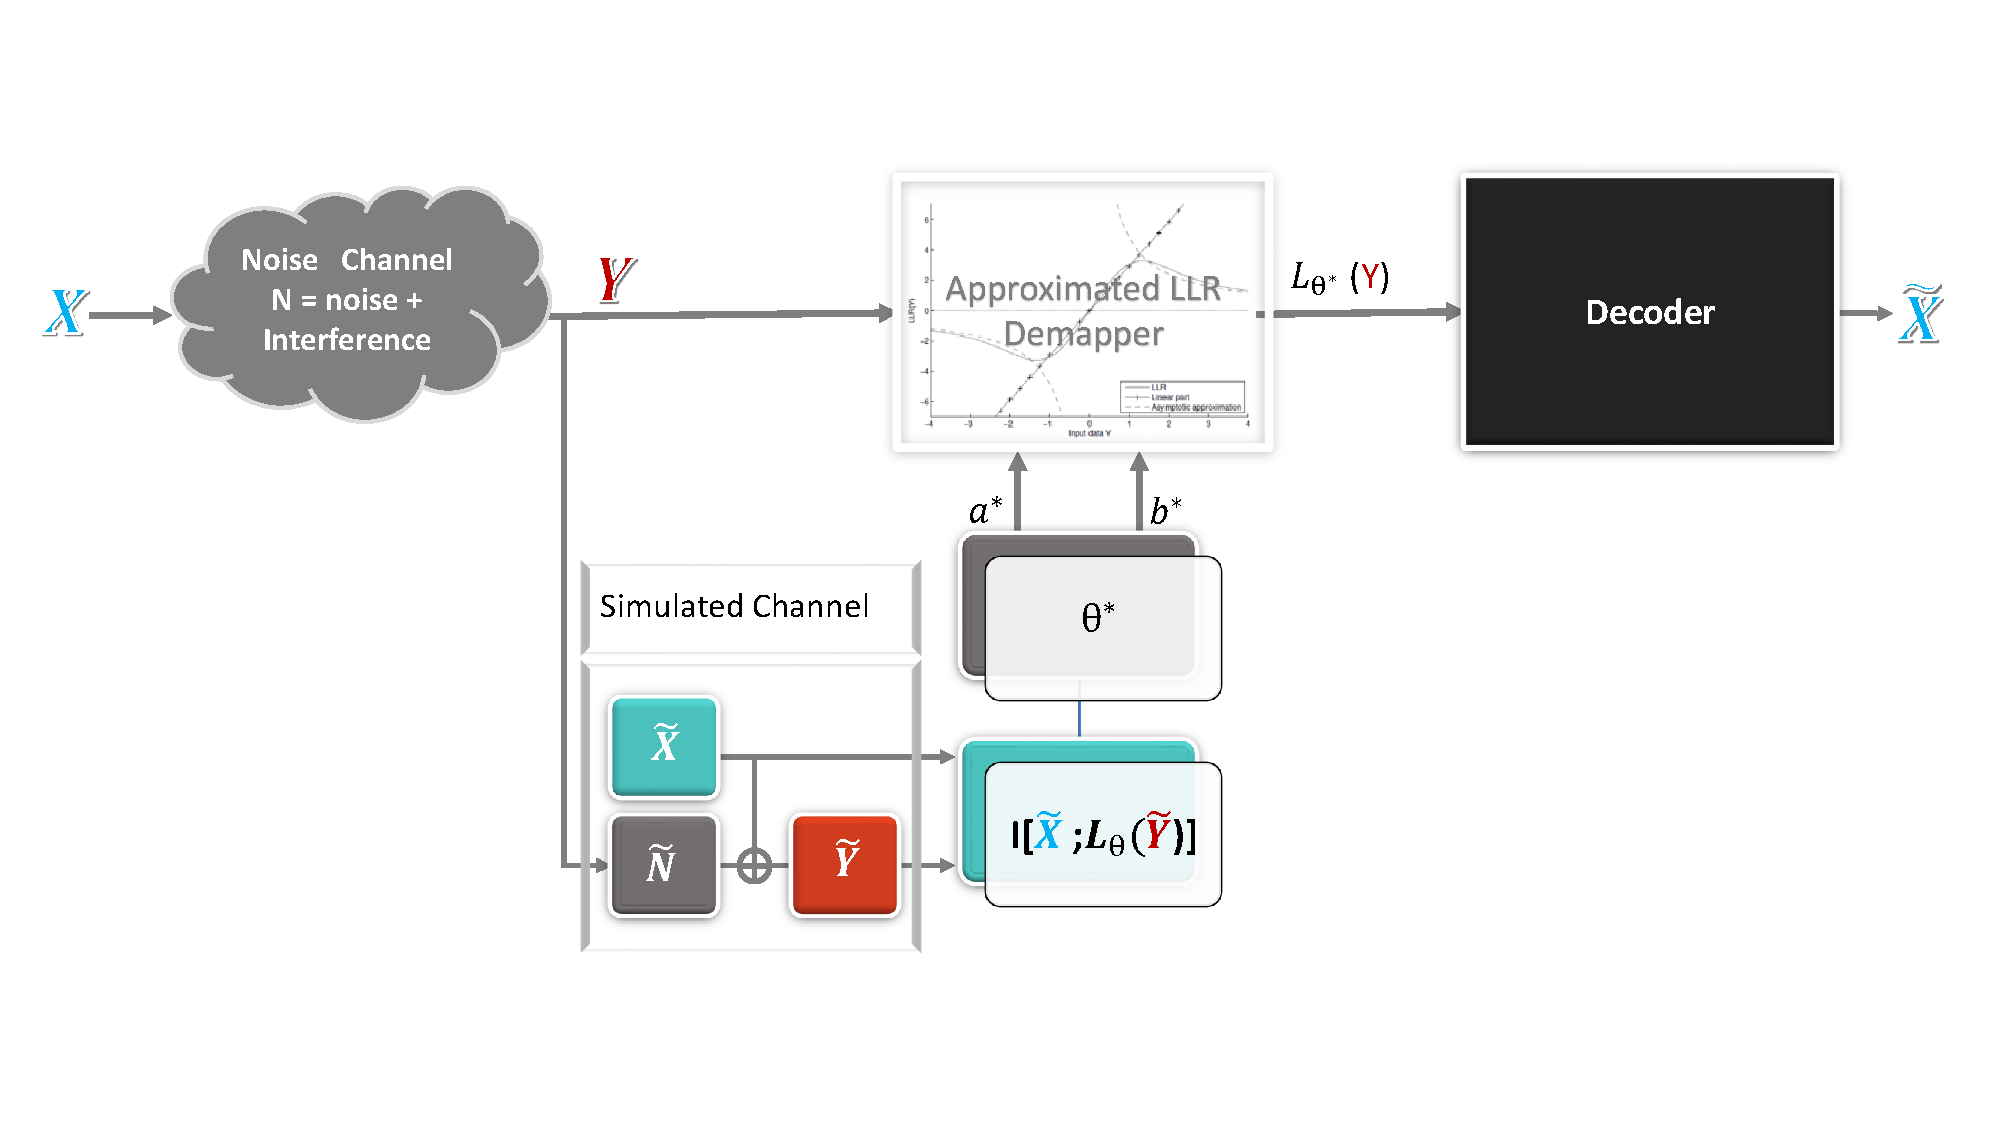
\includegraphics[width=\linewidth]{fig-5}
  \caption{Unsupervised LLR demapper.}
  \label{fig:5}
\end{figure}

Once the optimal parameters $\theta^*$ are obtained, the LLR
will be approximated by $L_{\theta^*}(Y)$.

\textcolor{red}{A: In the next Section, we propose to apply
  our blind LLR approximation optimization to LDPC coding
  where the noise exhibits an impulsive nature. }




\section{Application to LDPC coding used over additive impulsive noise}
\label{section:ldpc}

\textcolor{red}{A: In this Section, we will first present
  our simulation setup. Then, we will investigate the
  accuracy of the optimization process, evaluate the BER
  performance of our proposed blind optimized demapper under
  $S\alpha S$ noise. Finally, we will investigate the
  robustness of our proposed model by evaluating the BER
  performance under other noise models than $S\alpha S$. }



\subsection{Simulation setup}
\label{subsection:SimuSetup}


\subsubsection{Source}

To validate our approach we use a Low-Density Parity Check
(LDPC) code and a belief propagation (BP) decoding
algorithm. This case is well-suited to our proposal because
the LLR have to be estimated and fed to the BP algorithm.

The binary message $X$ is encoded using a regular (3,6) LDPC
code of length 20000. LDPC codes introduced by
Gallager~\cite{G-1963} and rediscovered by
Mackay~\cite{MN-1996} are powerful block codes due to their
near capacity performance under Gaussian noise. They are
widely used in various standards such as DVB-S2 and WiMAX.\@
Thanks to the sparseness of the parity check matrix of the
LDPC codes, the BP algorithm exhibits a quasi-linear
complexity as the code length growth.


\subsubsection{Noise}

Non Gaussian noises can arise in networks like it has been
shown many times. In the following we assume that the
additive noise impacting the transmission exhibits an
impulsive nature. In a first step, we will use Symmetric
$\alpha$-stable ($S\alpha S$) distributions to model this
impulsive interference, since the heavy tail property of
their pdf has been shown to coincide with the impulsive
nature of network interference in various environment
types~\cite{NHJ-2008, MPL-2009, HLNFP-2010, E-1992}.
Unfortunately, in general, no closed-form expression of its
pdf exists, which prevents the extraction of a simple metric
based on the noise pdf in the decoding algorithm. This is
precisely a case that can be solved by our proposal.

We also want to be model agnostic. Consequently we will
study the behavior of our approach with other classical
noise models: a simple Gaussian noise, a Middleton class
A and an $\epsilon$-contaminated.


\subsubsection{LLR approximation}

If the noise is Gaussian, the decoder's inputs (LLR) are
given as a linear function of the received signal $Y$. The
family of function should then simply be:
\begin{equation}
  L_{a}(y)=ay
\end{equation}
and $\theta$ is a single parameter, the slope $a$ of the
linear function. The optimal $\color{red}a^*$ in additive
white Gaussian noise channel only depends on the noise
variance as $L_{\color{red}a^*}(y)=\frac{2}{\sigma_N^2}y$.

Nevertheless, using only a linear scaling whose slope
depends on the additive noise variance leads to severe
performance loss as soon as noise is impulsive.

This performance loss occurs because with this linear
scaling, large values in $Y$ result into large LLR.\@
However, under impulsive noise, large values in $Y$ are more
likely due to an impulsive event so that the LLR should be
small, meaning a poorly reliable sample due to the presence
of a large noise sample.

\figurename~\ref{fig:3} lightens the non-linearity of the
LLR function for the channel output $Y$ when the noise is
$\alpha$-stable. Even if \figurename~\ref{fig:3} delineates
a specific noise model, the overall appearance of the LLR
exhibits a similar behavior when noise is impulsive.

\begin{figure}
  \centering 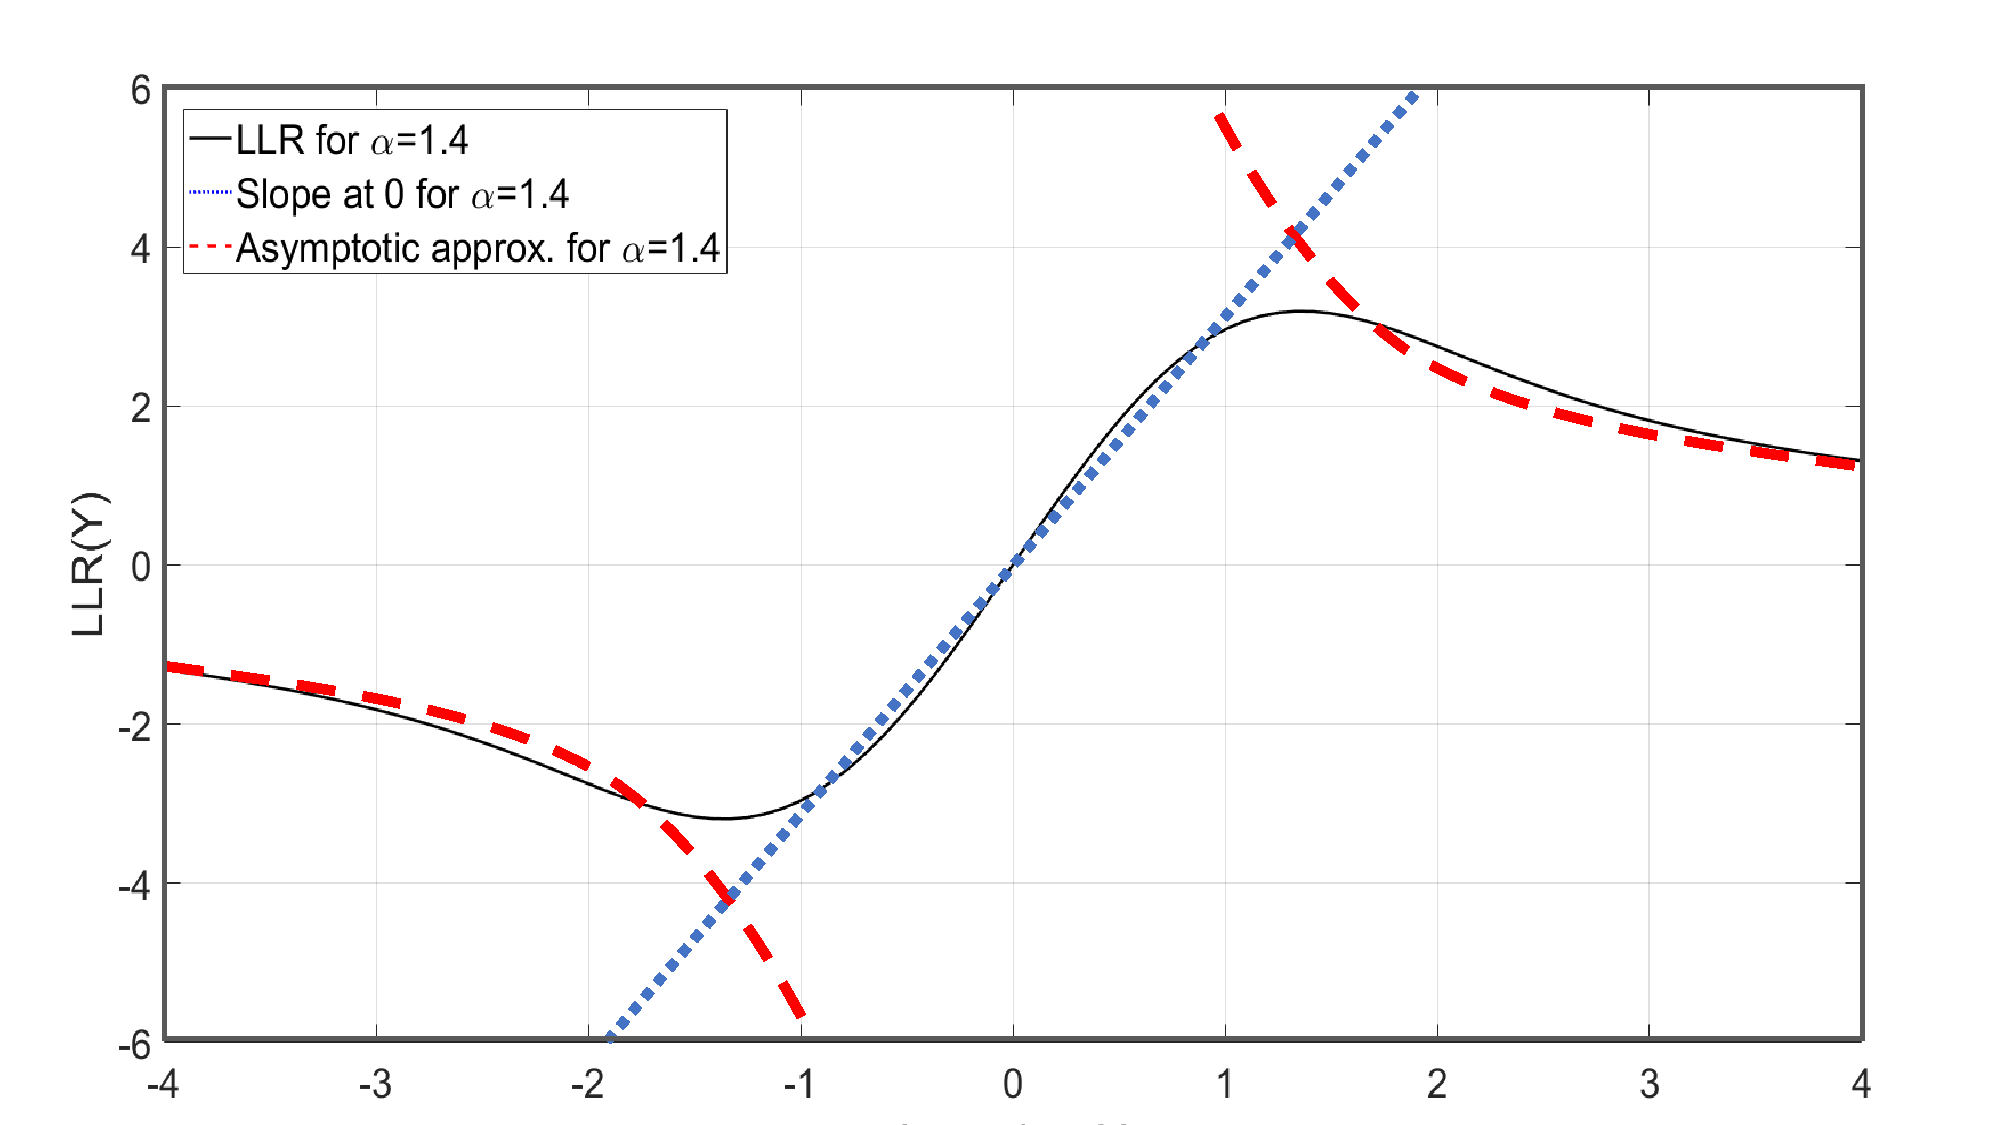
\includegraphics[width=\linewidth]{fig-3}
  \caption{LLR demapper for $\alpha=1.4$, $\gamma=0.5$, and
    its approximation.}
  \label{fig:3}
\end{figure}

At a first look, two different parts in the LLR can be
observed: a first one when $y$ is close to zero and another
one when $y$ becomes large enough. When $y$ is close to
zero, the LLR is almost linear, whereas when $y$ is large
enough, the LLR presents a power-law decrease. The linear
region spreads with the decrease of the noise impulsiveness
until reaching the limit (only the linear part exists), when
the noise is Gaussian. Several approximations taking into
account these two parts have been proposed~\cite{VALG-2014,
  SJD-1994, HALG-2013, SME-2012}. For illustration purposes,
we choose the LLR approximation family $L_{a,b}$ given in
\eqref{eq:12c}.



\subsection{Estimation in Additive S$\alpha$S Noise}


\subsubsection{Analysis}

In a first step, we investigate the shape of the function
$f_{\text{opt}}(a, b)$ in (\ref{eq:15}). In this paper we
present the obtained results for a highly impulsive noise
when $\alpha=1.4$, but the same observations and conclusions
can be made for \textcolor{red}{larger $\alpha$.}

\textcolor{red}{A: On \figurename~\ref{fig:12}, we represent
  a 3D plot of the function $f_{opt}(a,b)$ for three values
  of $\gamma$, namely $\gamma=0.35$, $\gamma=0.45$ and
  $\gamma=0.55$, as well as a contour plot representing the
  levels of $f_{opt}(a,b)$. First note that $f_{opt}$ is
  indeed a convex function, as was proven in Section
  NEEDREF, and that it is quite flat at its minimum value.
  Thus, the convergence of our blind optimization problem to
  its optimal $\theta^*$ is guarantied but it is quite
  sensitive to errors and thus to the length of the training
  sequence. Using the whole data set in an unsupervised
  approach can then be a source of robustness.}
\begin{figure*}
  \begin{multicols}{3}
    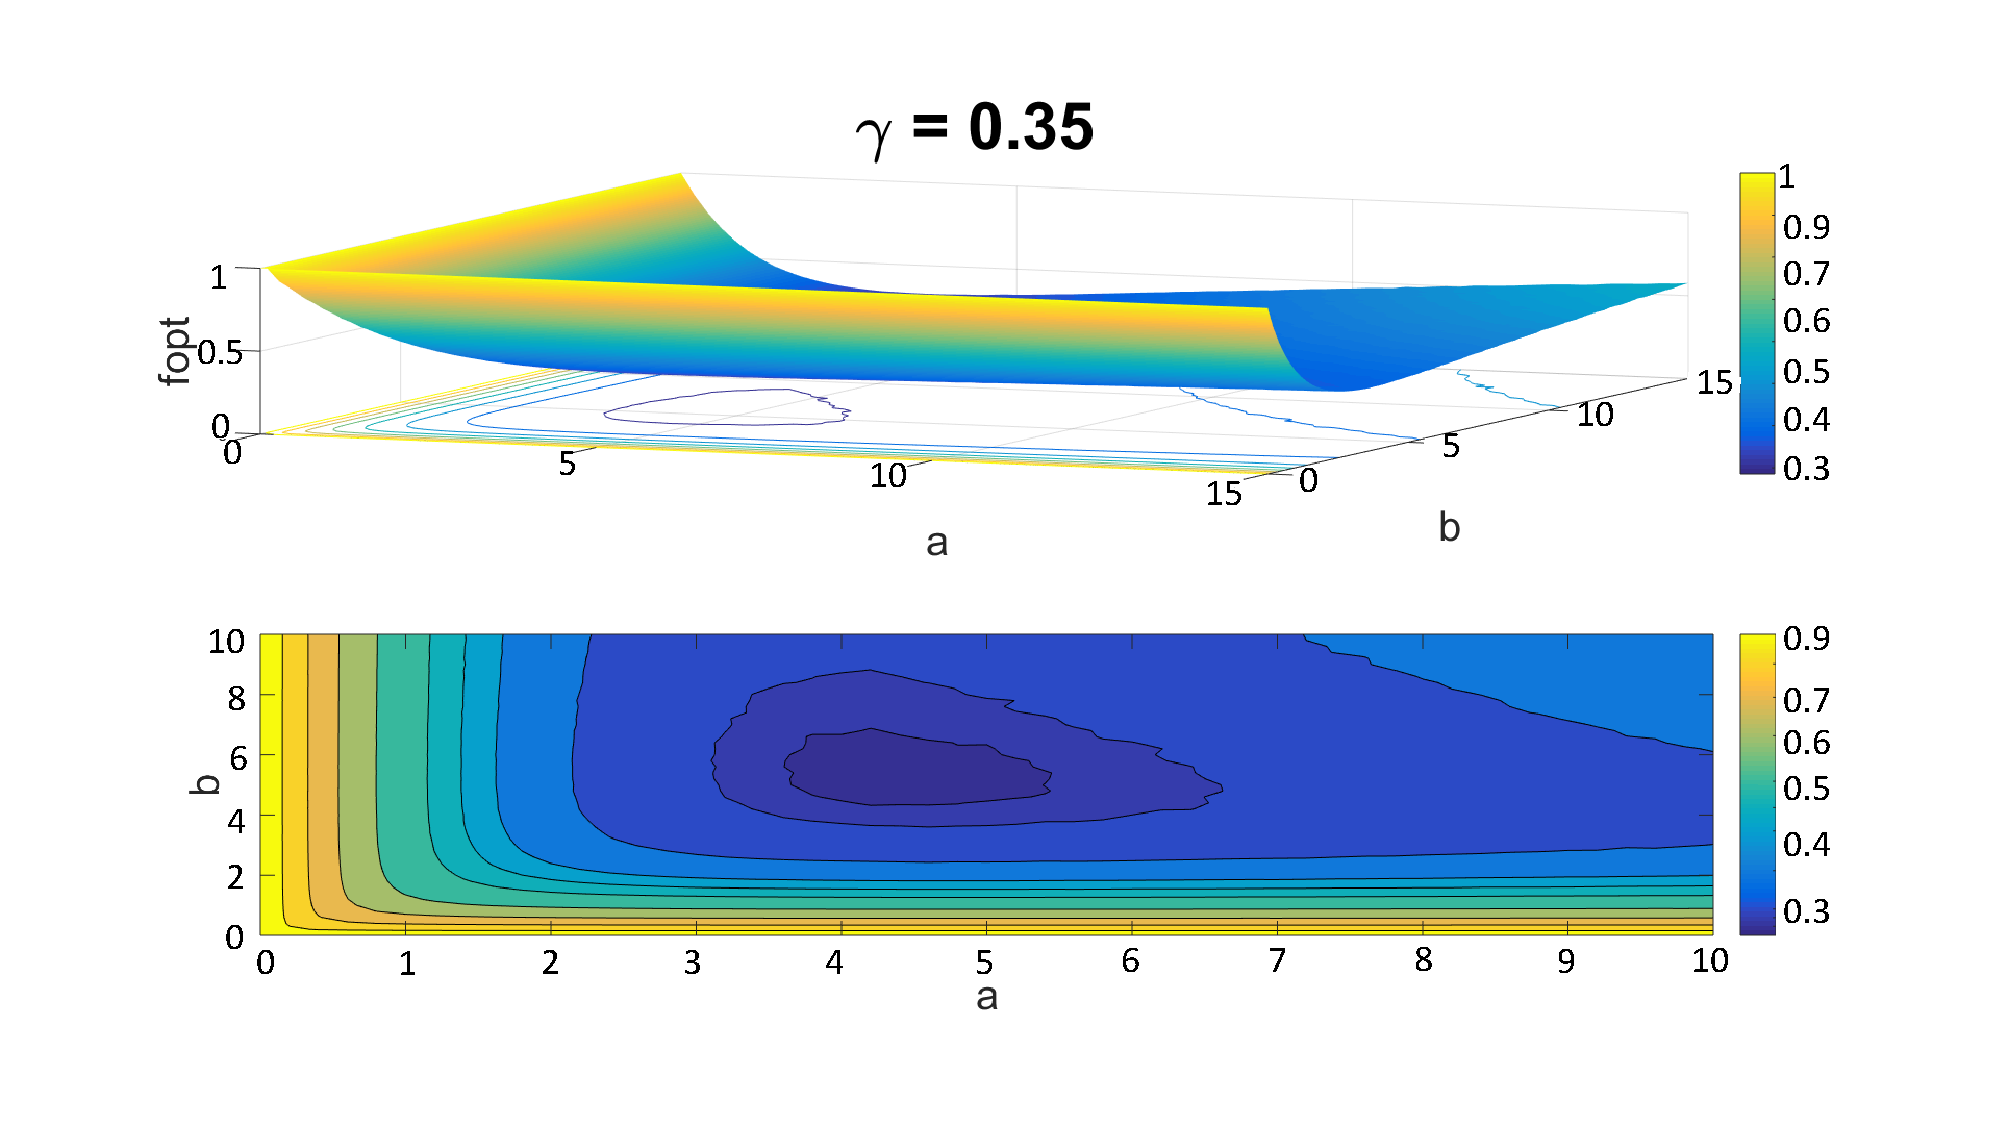
\includegraphics[height=0.3\textheight,width=1.05\linewidth]{fig-12a}\par
    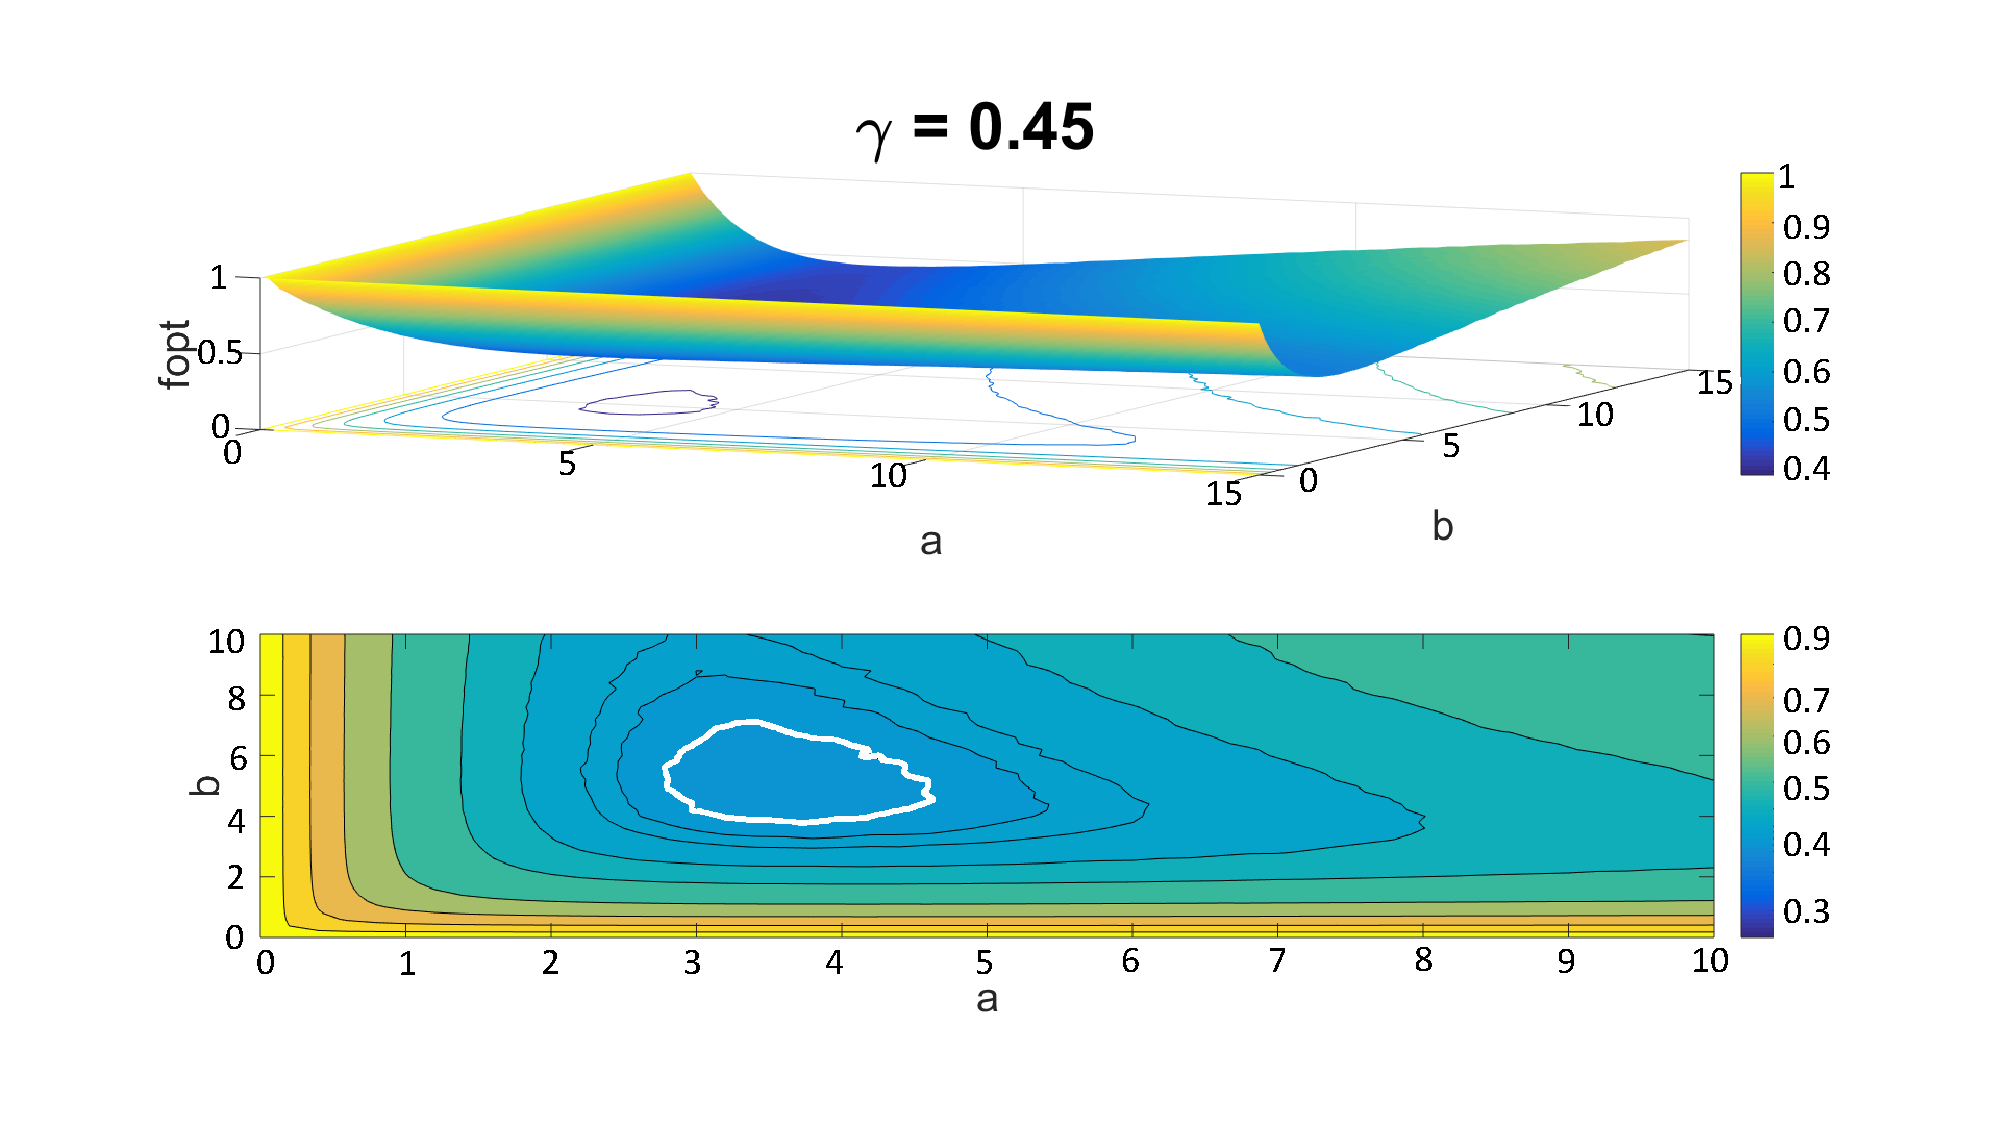
\includegraphics[height=0.3\textheight,width=1.05\linewidth]{fig-12b}\par
    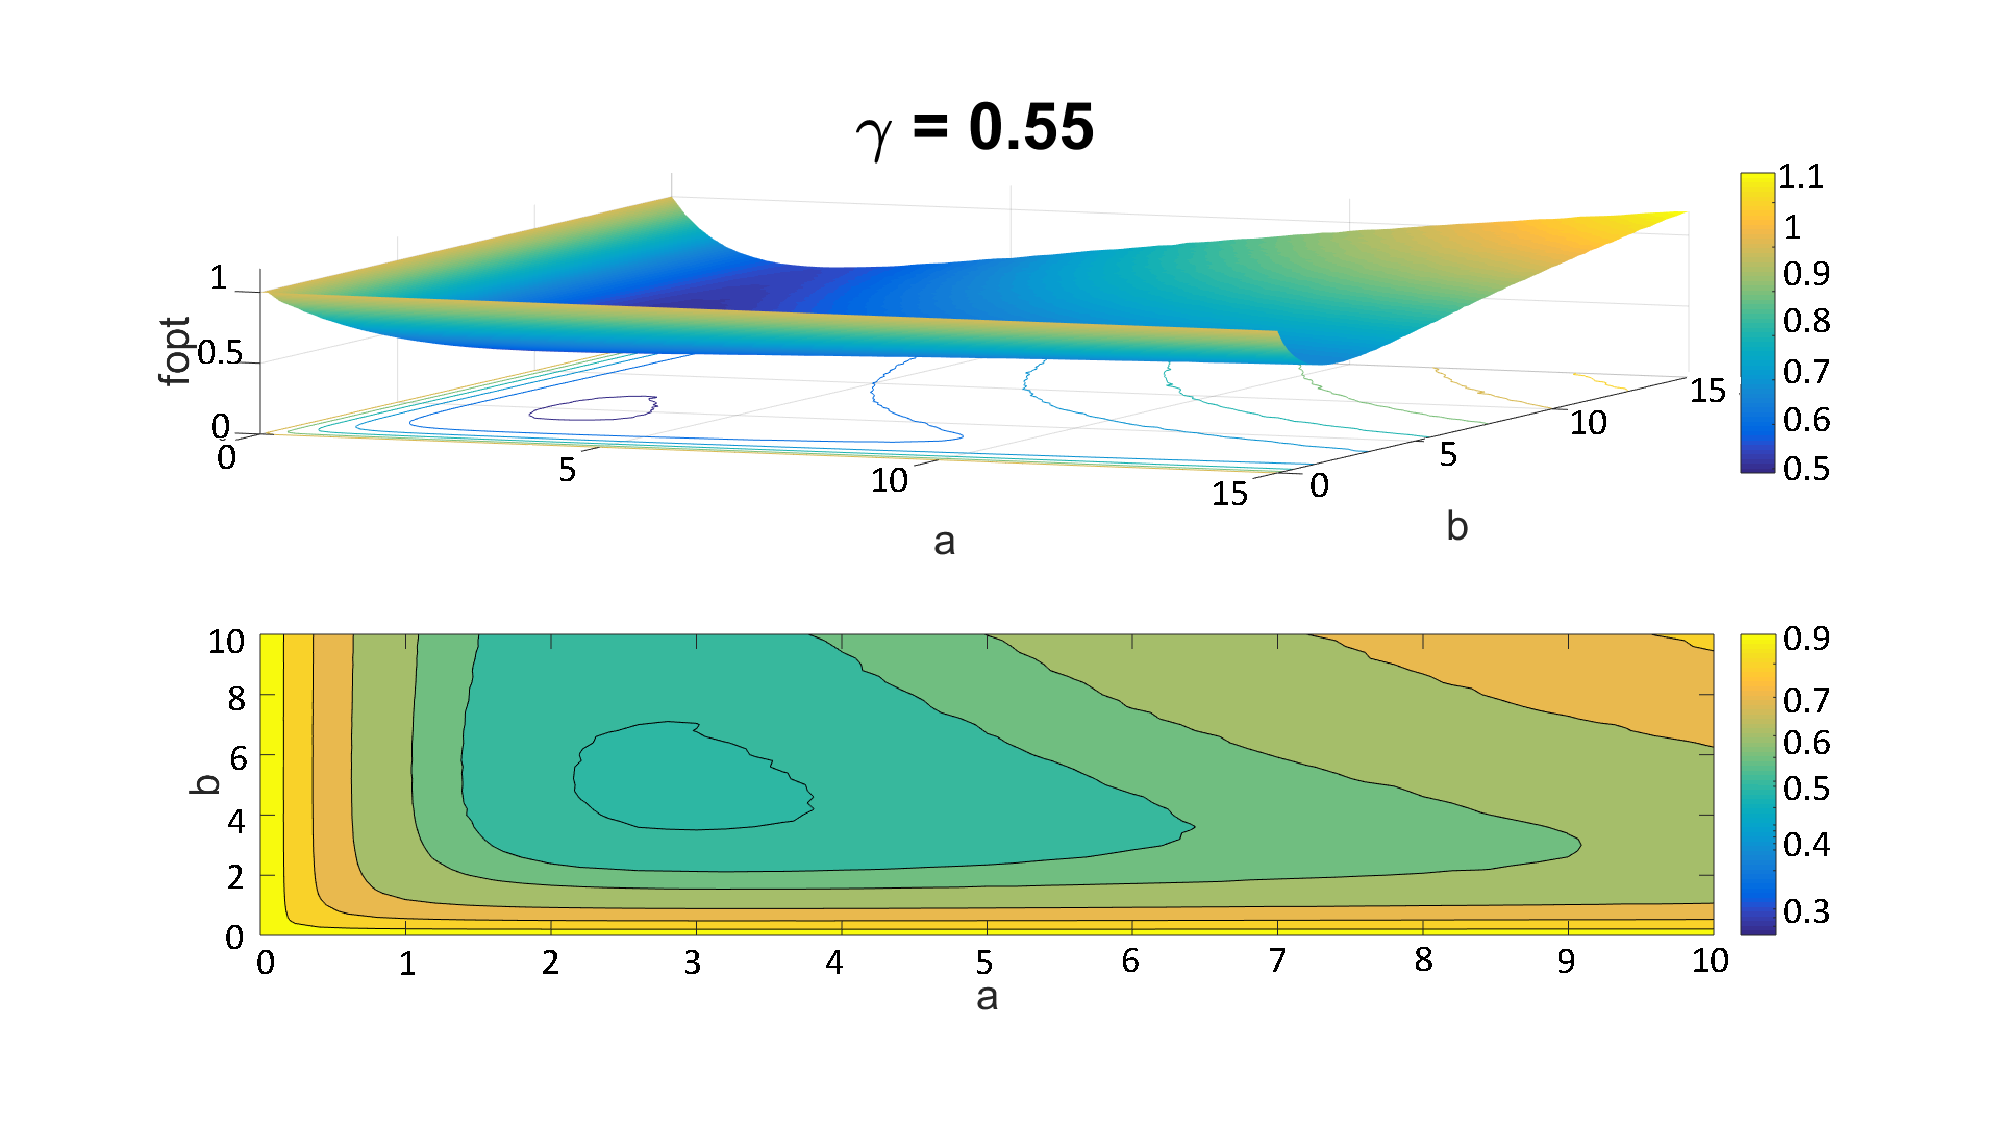
\includegraphics[height=0.3\textheight,width=1.05\linewidth]{fig-12c}\par
  \end{multicols}
  \caption{Behavior study of the $f_{opt}$ function, as a function of
    parameters $a$ and $b$ for different values of $\gamma$, under highly
    impulsive $S\alpha S$ noise with $\alpha =1.4$.}
  \label{fig:12}
\end{figure*}


\textcolor{red}{A: In \figurename~\ref{fig:13}, we
  illustrate the link between the function $f_{opt}$ and the
  obtained BER.\@ The contour plot delineates different BER
  values, ranging from $10^{-5}$ to $10^{-1}$, whereas the
  white contour delineates the set of $a$ and $b$ values
  yielding the smallest values of $f_{opt}$ within a small
  precision error. Note that the regions match in the sense
  that the set of optimal values for $a$ and $b$ allows the
  decoder to achieve a BER below $10^{-4}$.}

\begin{figure}
  \centering
  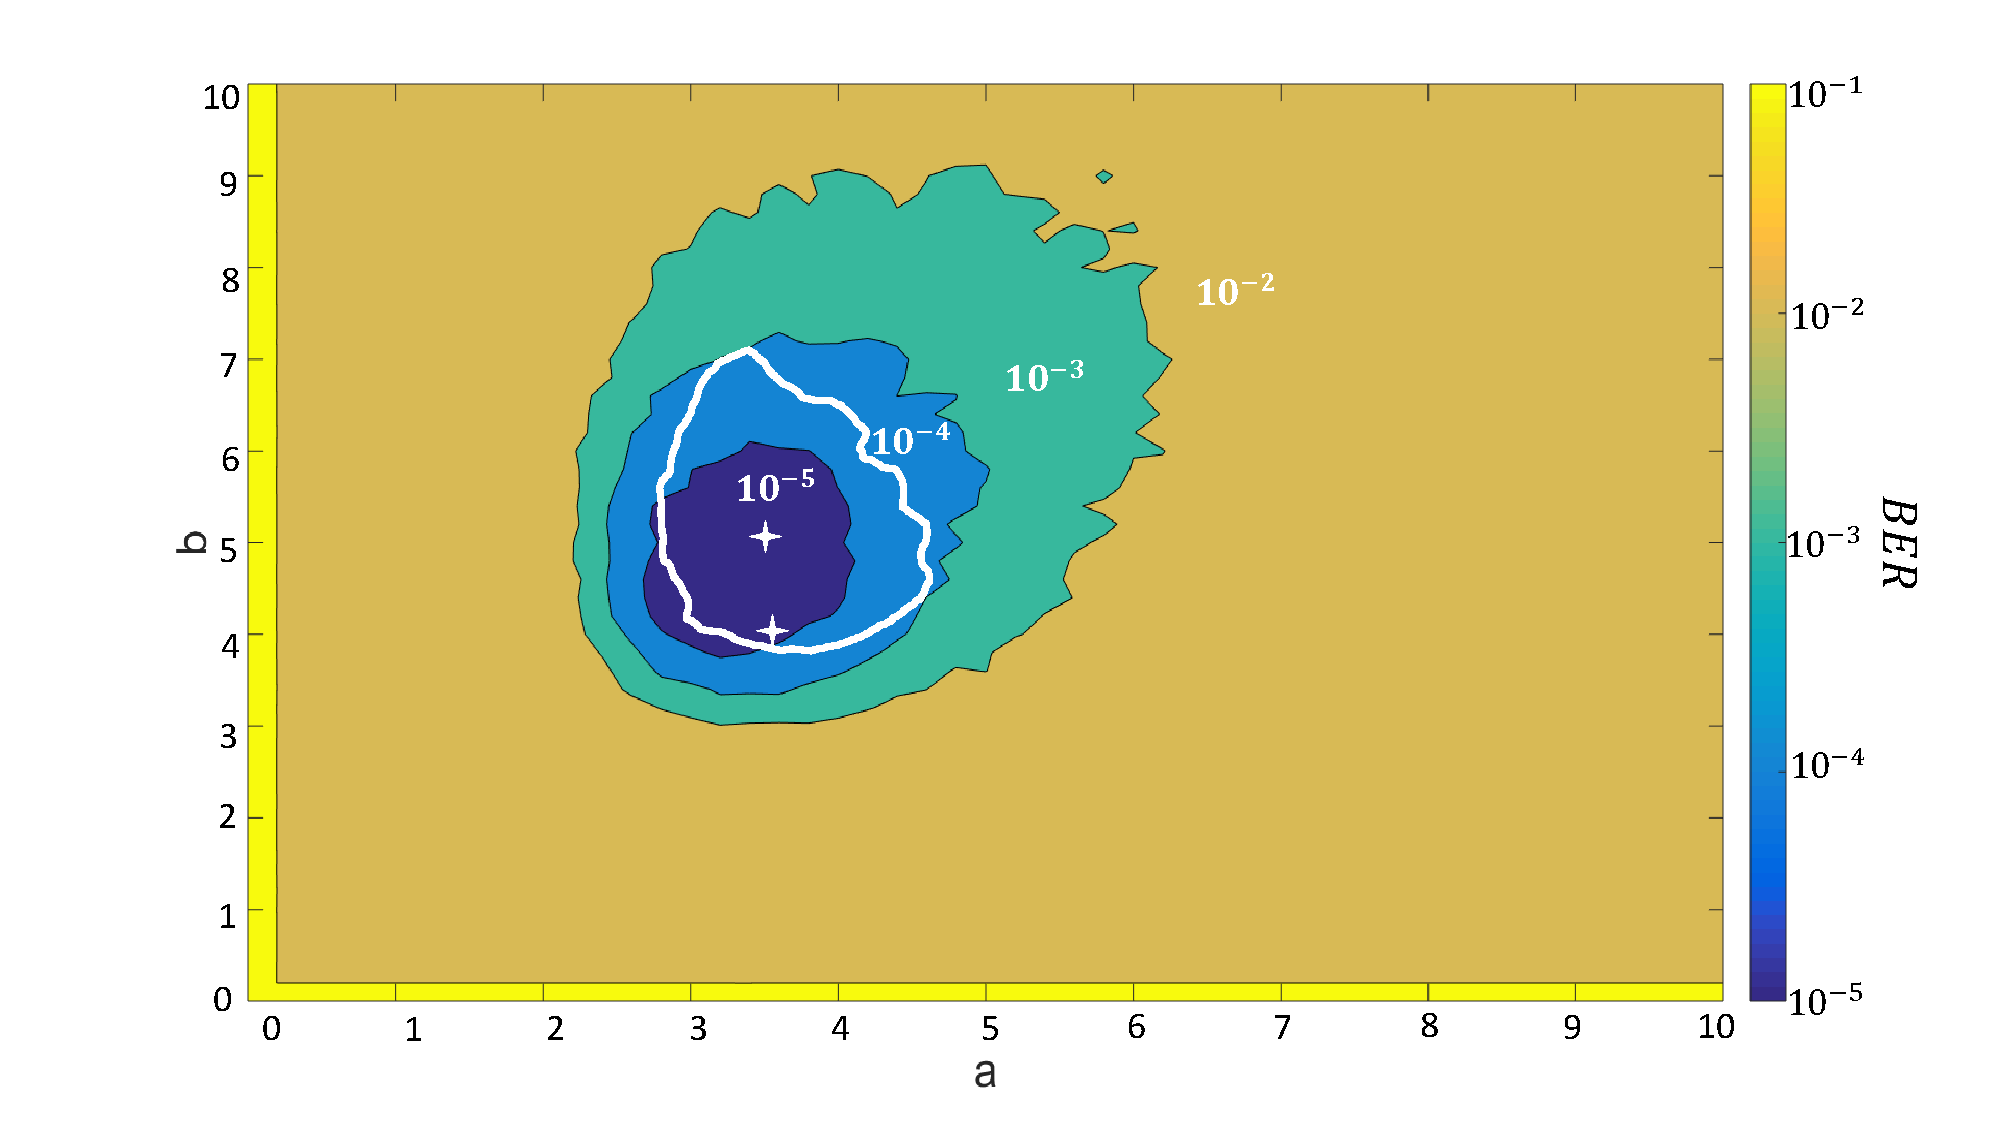
\includegraphics[width=\linewidth]{fig-13}
  \caption{BER comparison as a function of $a$ and $b$
    parameters with $\gamma = 0.45$ and $\alpha=1.4$ under
    the supervised approximation.}
  \label{fig:13}
\end{figure}

\textcolor{red}{A: We will next evaluate the performance of
  the estimation process. To perform so, we compare the
  obtained $\theta^*$ under blind optimization with the one
  obtained under a supervised approach. In the later,
  instead of building a training sequence $\widetilde{X}$ at
  the decoder, we directly use the learning sequence to
  estimate the optimal $\theta^*$. More details on the
  supervised optimization can be found in our
  paper~\cite{NEEREF}.}


\subsubsection{Estimation performance}\label{subsection:EstSaS}

\figurename~\ref{fig:7}, respectively
\figurename~\ref{fig:8}, compares the evolution of the mean
and variance of the estimated parameter $a$, respectively
$b$, as a function of the dispersion $\gamma$ of a $S\alpha
S$ noise with $\alpha=1.4$ under supervised and unsupervised
optimization. For each noise dispersion, we ran 100
experiments. For the supervised case, we use a learning
sequence of 20000 samples to estimate $a$ and $b$. This
allows to have a good idea of the results with a very small
estimation error but, in a practical setting, such a long
training sequence is not reasonable and additional errors
can be expected \textcolor{red}{A: as the length of the
  learning sequence decreases.}

\begin{figure}
  \centering
  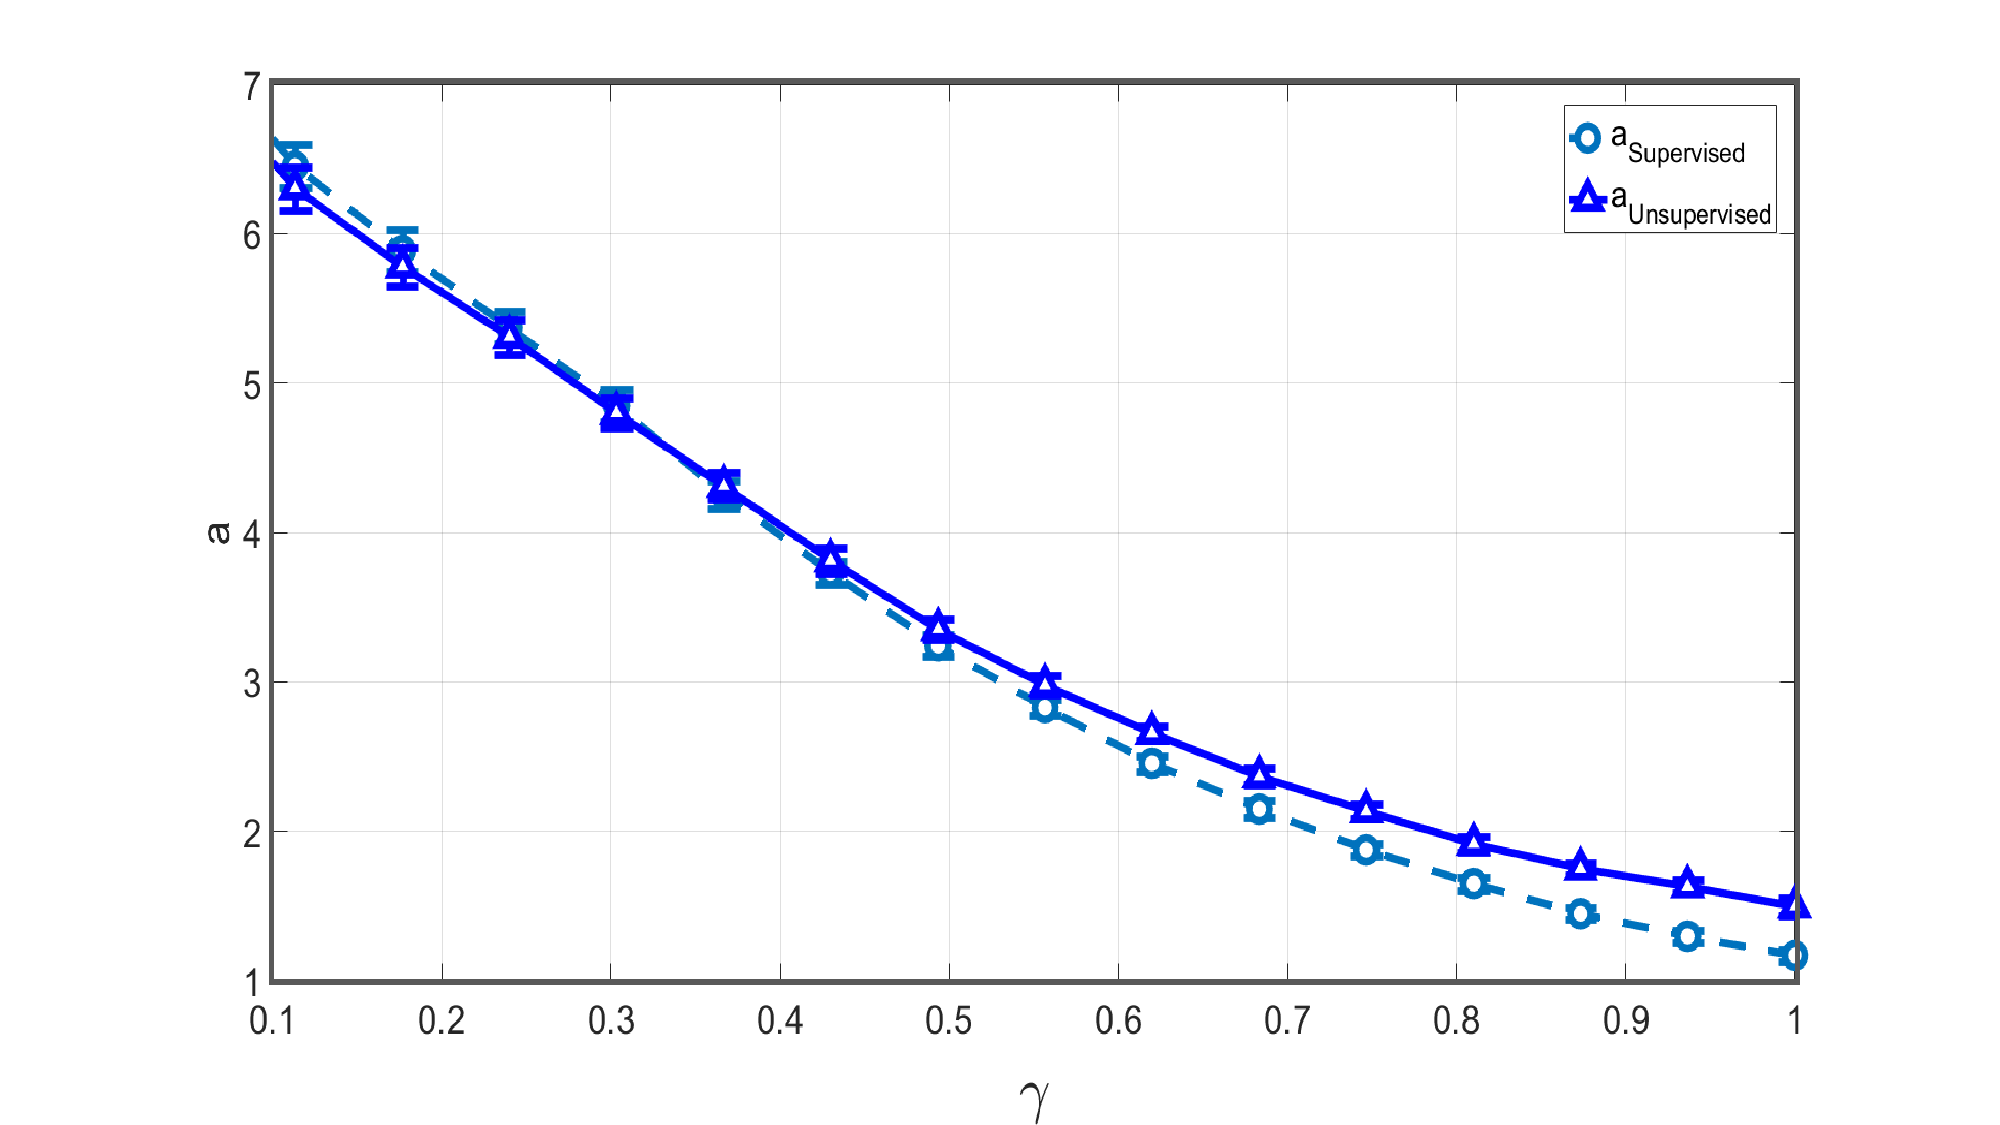
\includegraphics[width=\linewidth]{fig-7}
  \caption{Comparison of the mean and standard deviation
    evolution for parameter $a$ as a function of the
    dispersion $\gamma$ of a S$\alpha$S noise with
    $\alpha=1.4$ for the supervised and unsupervised
    optimization.}
  \label{fig:7}
\end{figure}

\begin{figure}
  \centering 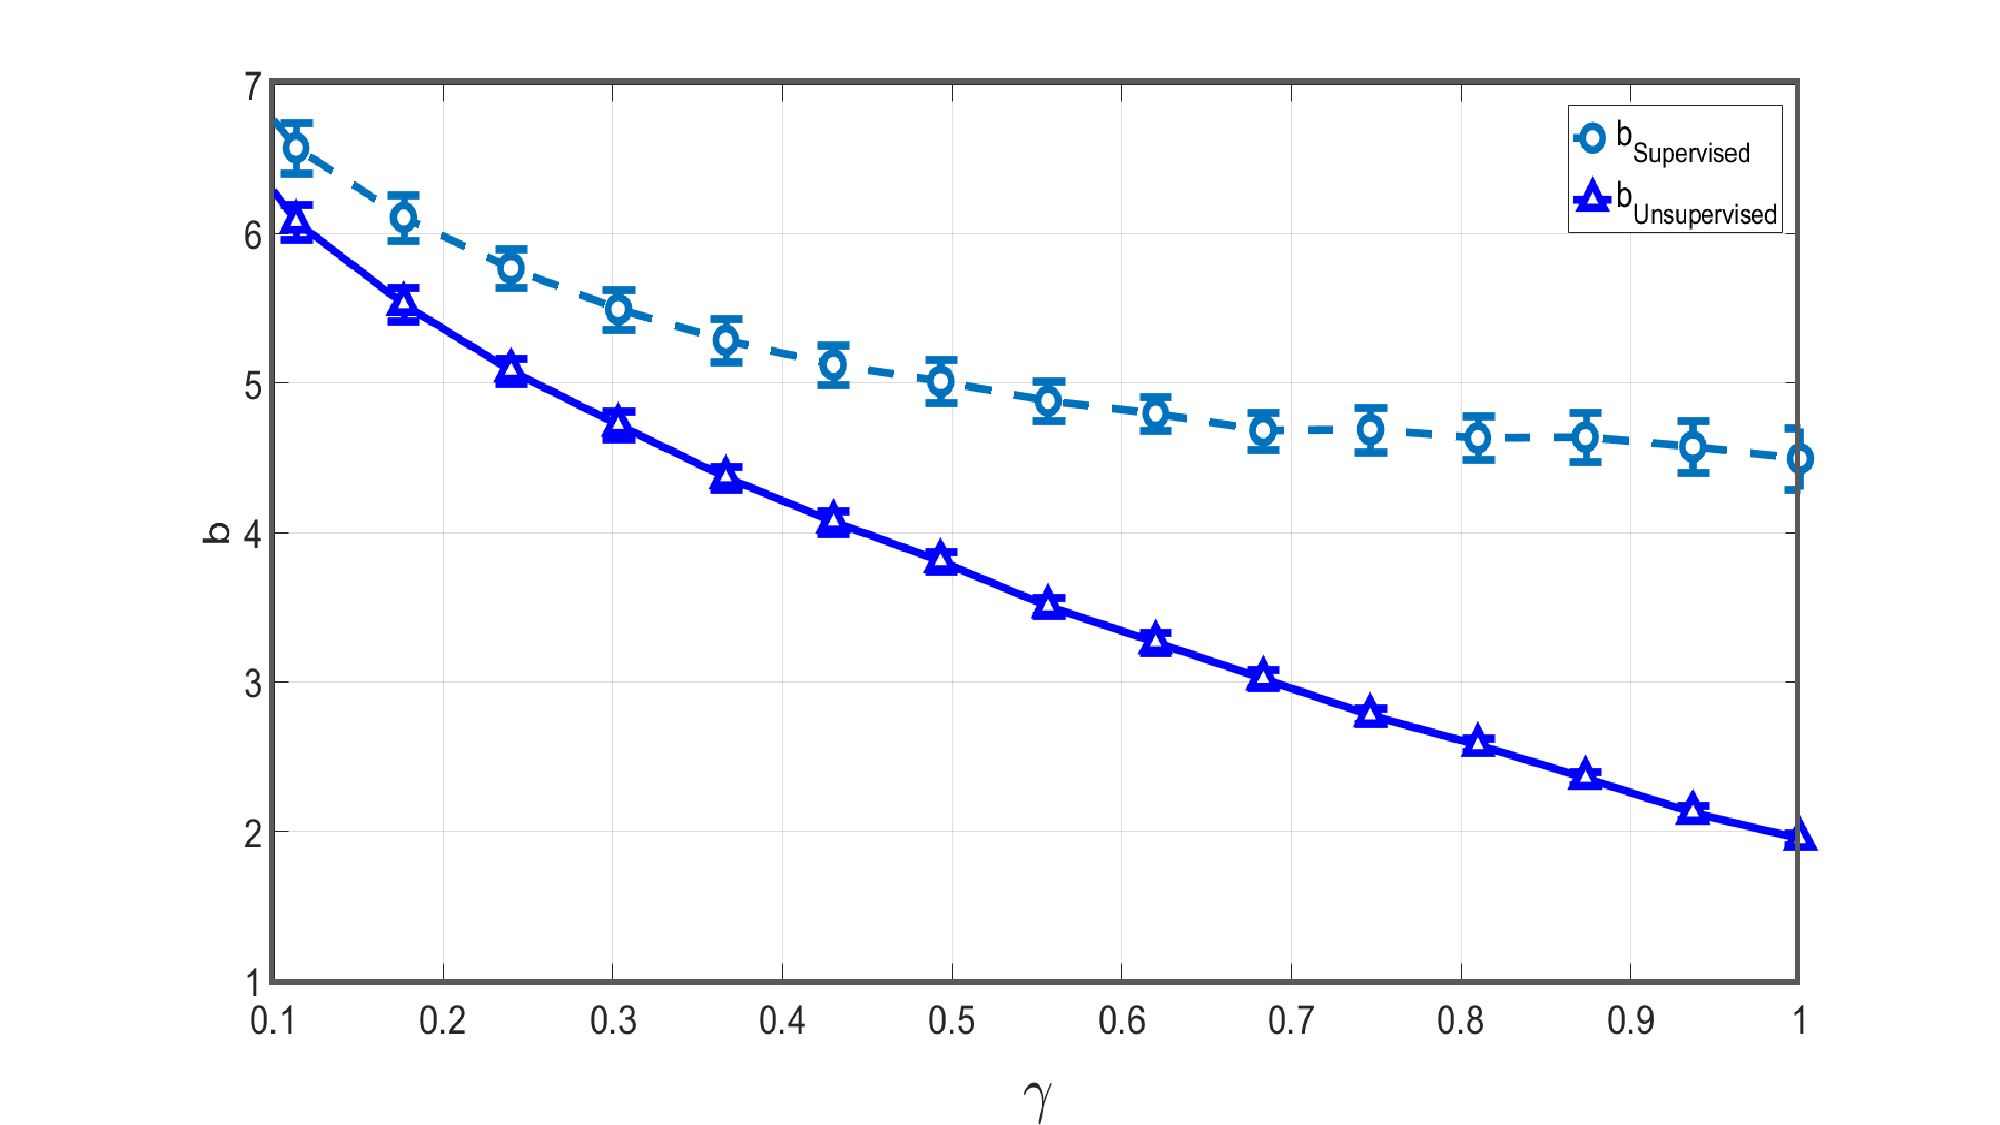
\includegraphics[width=\linewidth]{fig-8}
  \caption{Comparison of the mean and standard deviation
    evolution for the parameter $b$ as a function of the
    dispersion $\gamma$ of a S$\alpha$S noise with
    $\alpha=1.4$ for the supervised and unsupervised
    optimization.}
  \label{fig:8}
\end{figure}

\textcolor{red}{A: We can see from \figurename~\ref{fig:7}
  that the gap between the obtained values for parameter $a$
  under supervised and unsupervised optimization is small.
  Unfortunately, as shown in \figurename~\ref{fig:8}, the
  one obtained for $b$ is significantly larger. This
  difference can be explained since $b$ mainly depends on
  large noise samples which are rare events; consequently,
  its estimation is less accurate. }

\textcolor{red}{A: We can however expect that the error on
  $b$ will have a limited impact in terms of BER
  performance. Indeed, as shown in \figurename~\ref{fig:13}
  when $\gamma=0.45$, both $a$ and $b$ estimated mean values
  under both the supervised and the blind approach fall in
  the small BER region. Besides, the small variance of the
  estimated $\theta^*$ ensures that most of the estimated
  values will fall in the region, yielding the smallest
  BER.}


To complete the study we present in Table~\ref{tab:a} the
influence of the training sequence length. The variance in
$a$ and $b$ gets large when the training sequence gets
short. This will probably influence the performance of the
system and degrade the BER.

\begin{table*}
  \begin{tabularx}{\linewidth}{ccc||CCCC||}
    \toprule \multicolumn{3}{c||}{} & \cellcolor{LightCyan}$\mu_{a}$ & \cellcolor{LightCyan}$\sigma_{a}$& \cellcolor{LightCyan}$\mu_{b}$ & \cellcolor{LightCyan} {}$\sigma_{b}$ \\
    \addlinespace \midrule \multirow{8}{4em}{$\alpha=1.8$}&
    \multirow{4}{4em}{$\gamma=0.53$}
    & $\text{Unsupervised}$       & 3.43    & 0.06                                & 5.73          & 0.15 \\
    &  &$\text{Sup}_{\text{LS=20000}}$ & 3.25    & 0.05                             & 7.59       & 0.28 \\
    &  &$\text{Sup}_{\text{LS=1200}}$  &  3.27    &   0.24     & \cellcolor{lightGray}  8.50       & \cellcolor{Gray} 14.48\\
    &  &$\text{Sup}_{\text{LS=900}}$   &  3.27    &   0.27          & \cellcolor{Gray}  11.72      & \cellcolor{Gray} 46.15\\
    \addlinespace &\multirow{4}{4em}{$\gamma=0.55$}
    &$\text{Unsupervised}$      & 3.23    & 0.05                                  & 5.61          & 0.14 \\
    &  &$\text{Sup}_{\text{LS=20000}}$ & 3.05    & 0.05                              & 7.62      & 0.28 \\
    &  &$\text{Sup}_{\text{LS=1200}}$  &  3.07   &0.22         & 7.97      & \cellcolor{lightGray} 1.54\\
    &  &$\text{Sup}_{\text{LS=900}}$   &  3.07   &  0.26             &  \cellcolor{Gray} 10.73    & \cellcolor{Gray} 30.41\\
    \addlinespace\bottomrule
  \end{tabularx}
  \caption{Comparison of the mean and standard deviation
    evolution for the parameters ($a, b$) as a function of
    the dispersion $\gamma$ of a S$\alpha$S noise with
    $\alpha=1.8$ for the supervised with different learning
    sequences and unsupervised optimization.}
  \label{tab:a}
\end{table*}


\subsection{BER performance \textcolor{red}{under $S\alpha S$ additive noise}}
\label{subsection:BERSaS}

Once our demapper is tuned with the estimated value
$\theta$, it is used as a front-end to the 20000 bits long
regular (3,6) LDPC decoder using the BP algorithm over an
additive impulsive $S\alpha S$ noise. We study a highly
impulsive situation with $\alpha= 1.4$ and a more moderate
case with $\alpha=1.8$.

\figurename~\ref{fig:10} and \figurename~\ref{fig:11}
present the obtained BER for $\alpha=1.4$ and $\alpha=1.8$
respectively, as a function of the dispersion $\gamma$ of
the $\alpha$-stable noise\footnote{In case of an impulsive
  environment with $\alpha < 2$, the second-order moment of
  a stable variable is infinite~\cite[Theorem 3]{NHJ-2008},
  making the conventional noise power measurement infinite.
  Accordingly, we present our simulation results as
  a function of the dispersion parameter $\gamma$, which is
  used as a measurement of the strength of the
  $\alpha$-stable noise.}. In both cases, we compare the BER
obtained via the demapping function, either in a blind or
supervised manner, to the BER obtained with the true LLR
computed via numerical integration. For each channel set, we
use a learning sequence of length (1200 or 20000) to
optimize $\theta$ in the supervised case; the long training
sequence (20000) allows to assess the optimal performance of
the supervised estimation, the shorter one (1200) allows to
evaluate the loss due to estimation with more realistic
training sequences.

\begin{figure}
  \centering 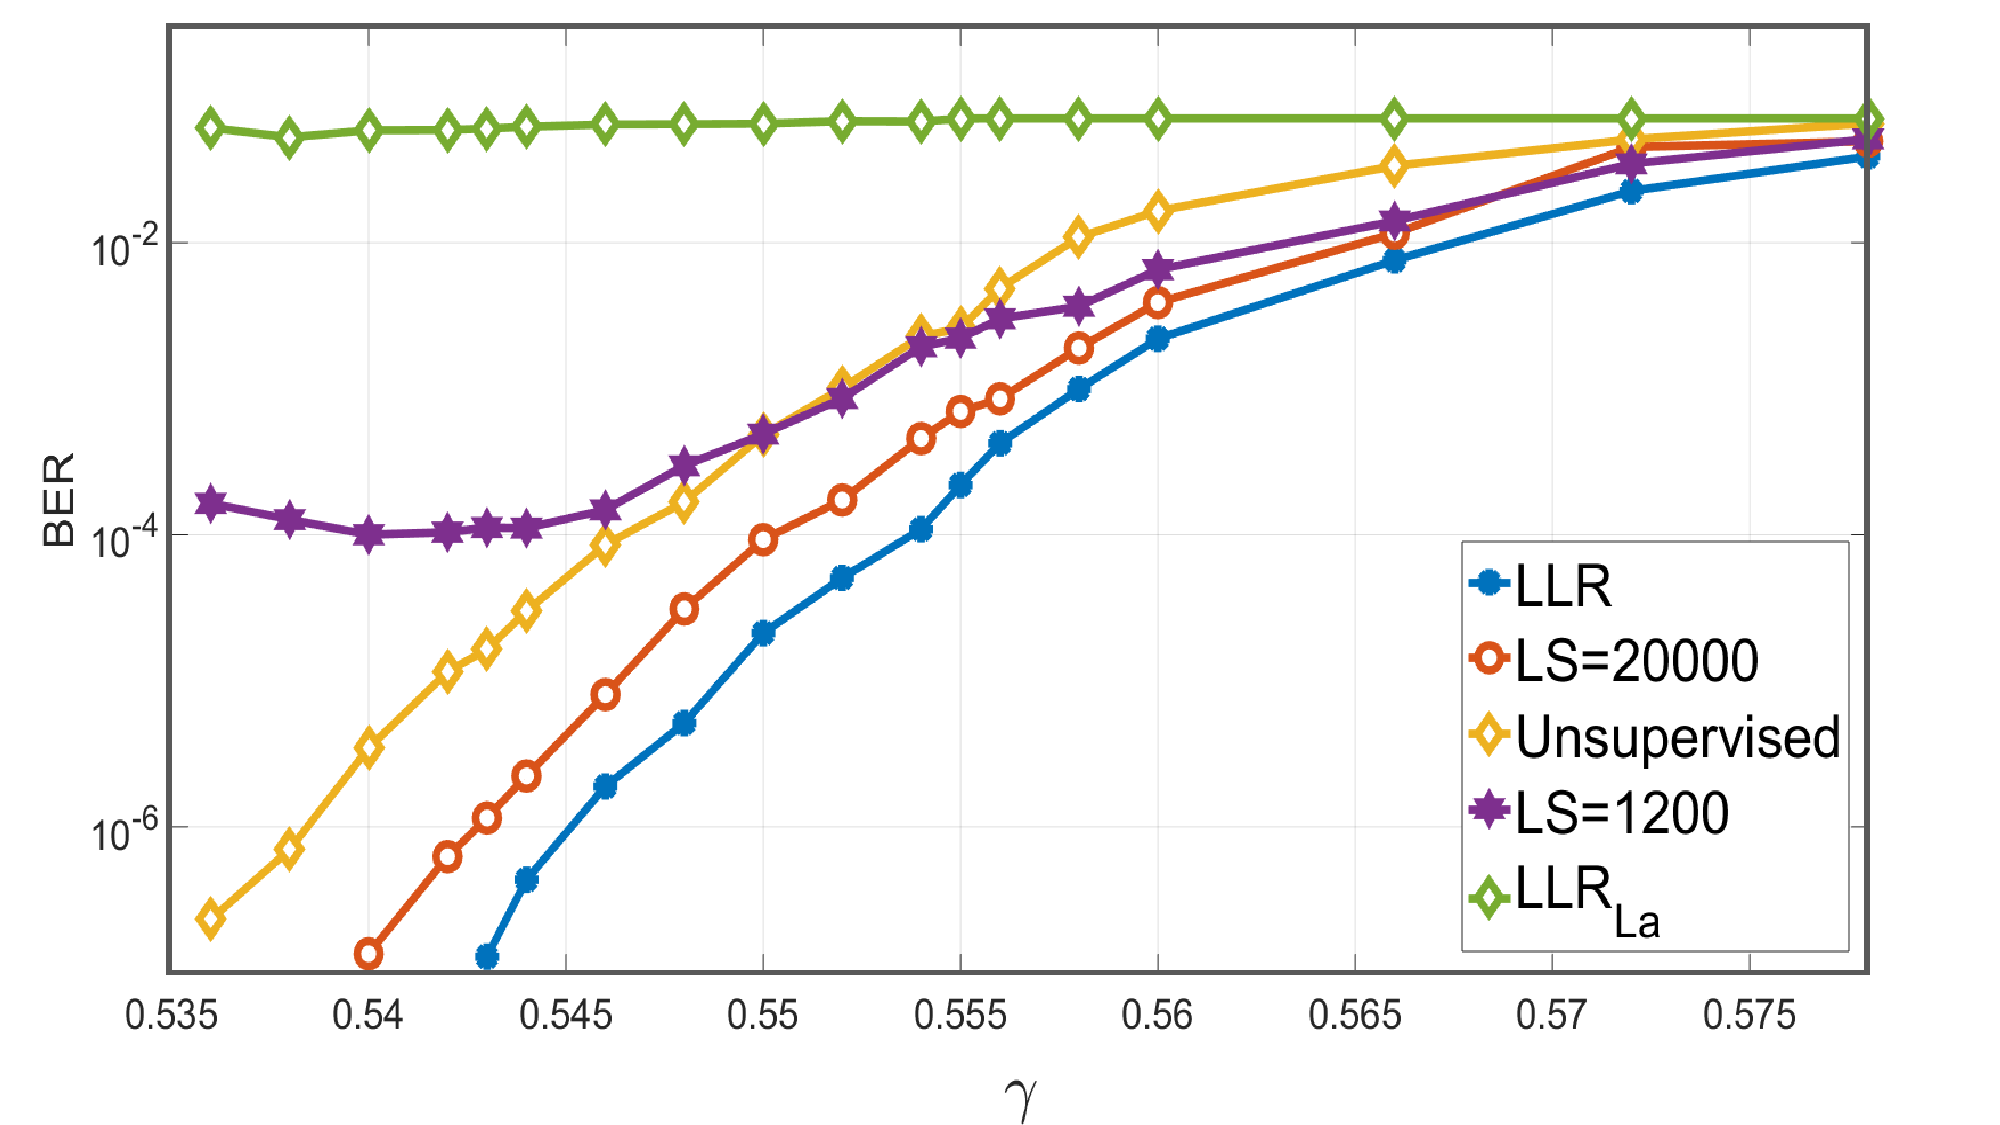
\includegraphics[width=\linewidth]{fig-10}
  \caption{Evolution comparison of the BER as a function of
    the dispersion $\gamma$ of a S$\alpha$S noise in poorly
    impulsive environment with $\alpha=1.8$, between the
    supervised with different learning sequence sizes,
    unsupervised, Gaussian designed LLR approximations and
    the LLR obtained by numerical integration.}
  \label{fig:10}
\end{figure}

\begin{figure}
  \centering 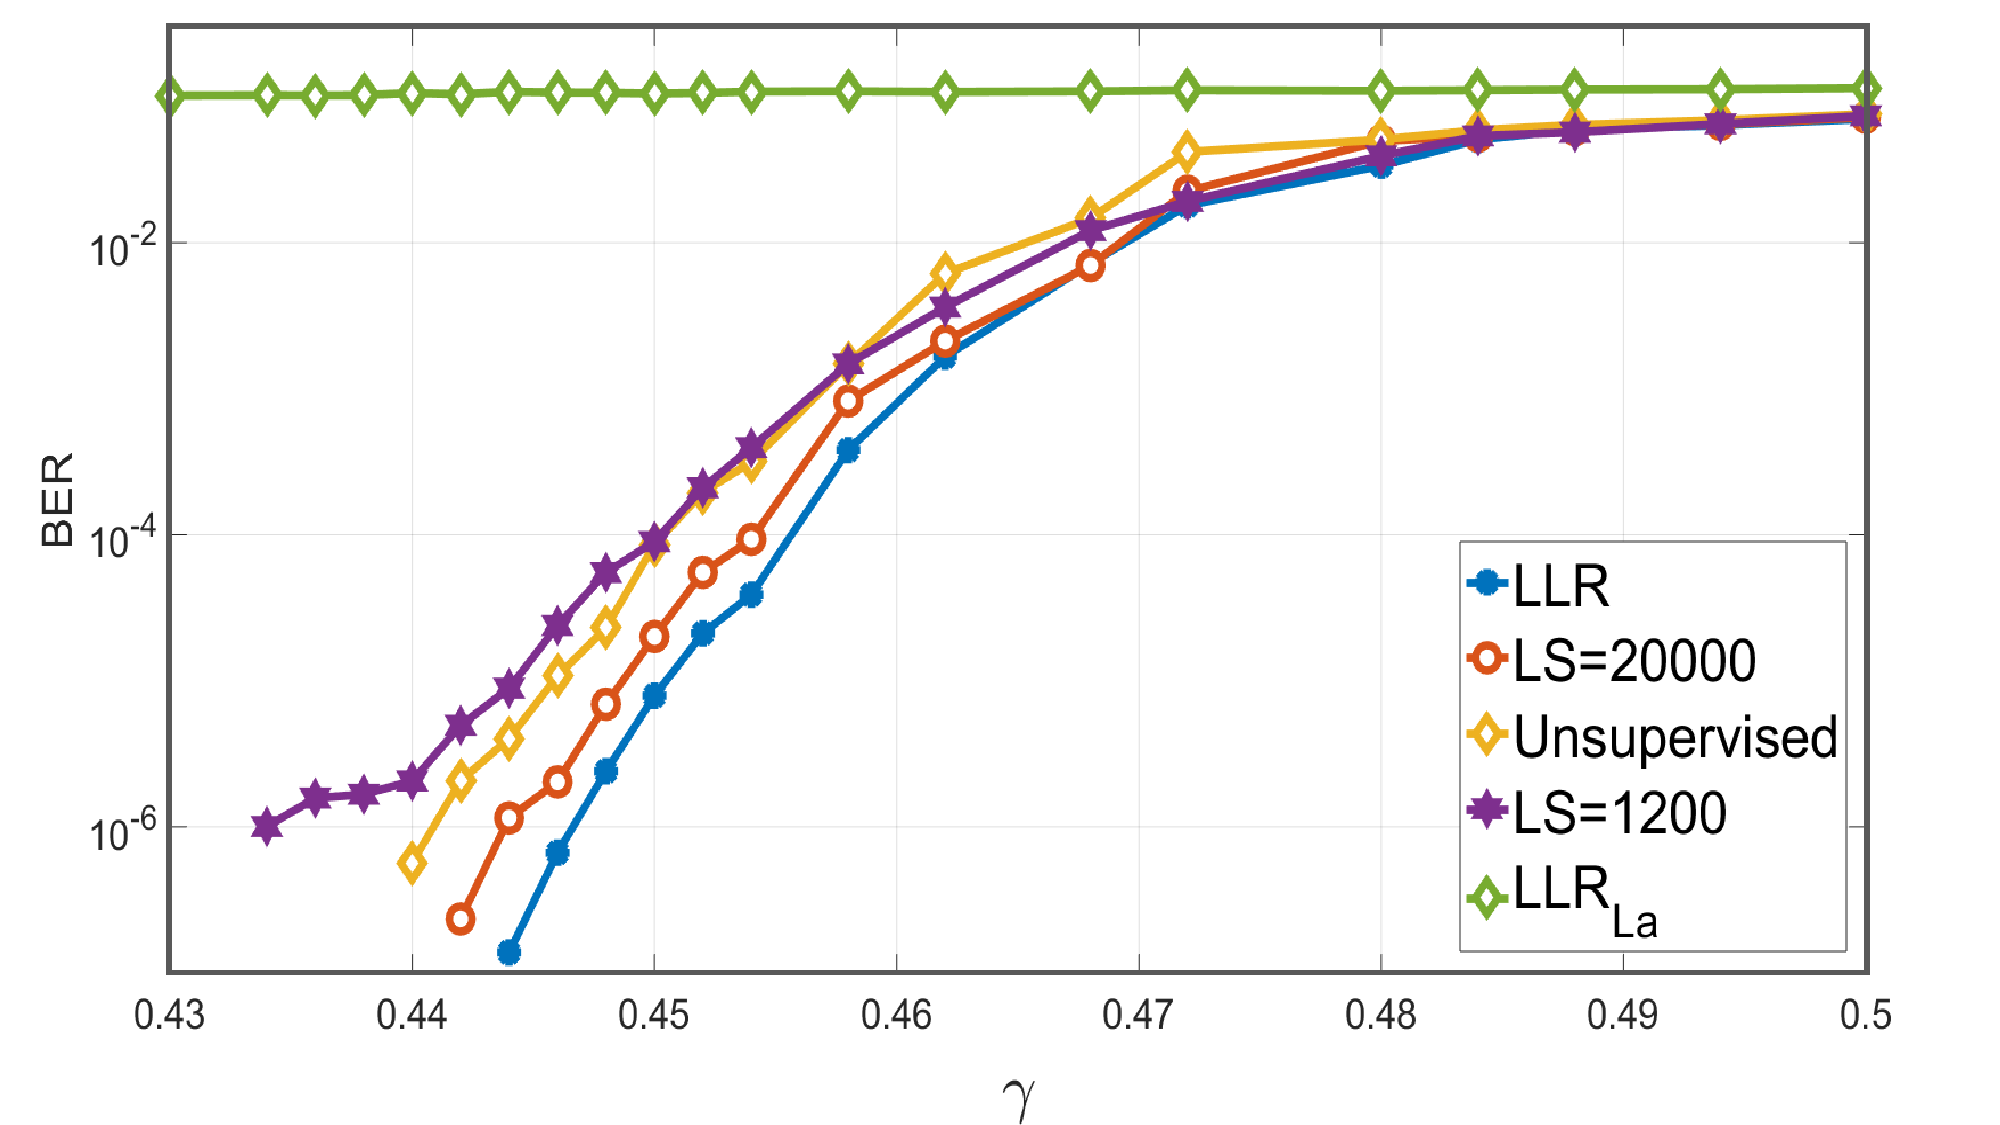
\includegraphics[width=\linewidth]{fig-11}
  \caption{Evolution comparison of the BER as a function of
    the dispersion $\gamma$ of a S$\alpha$S noise in highly
    impulsive environment with $\alpha=1.4$, between the
    supervised with different learning sequence sizes,
    unsupervised, Gaussian designed LLR approximations and
    the LLR obtained by numerical integration.}
  \label{fig:11}
\end{figure}

First, we note that the estimation with a long training
sequence gives performance close to the optimal LLR which
shows the good behavior of our demapping function. Moreover,
the unsupervised approach does not perform as well as the
supervised one with long training sequence but the gap is
not so large and the gain in comparison to a linear receiver
is enormous. However, when the training sequence is
shortened, the supervised estimation degrades and the
performance of the blind approach is then much better.

\textcolor{red}{In order to show the robustness of our
  proposed demapper $L_{a,b}$, we investigate in the next
  Subsection its performance when instead of suffering from
  a $S\alpha S$ noise, the channel exhibits either an
  impulsive nature, modeled by Middelton Class
  A~\cite{AD-1977} or $\varepsilon$-contaminated
  noises~\cite{Alhussein2017}, or a Gaussian one.}



\subsection{Robustness study of the proposed LLR approximation}
\label{subsection:Robustness}


\subsubsection{Other additive impulsive noise channels}

\textcolor{red}{A: We start by considering two other models
  of impulsive noise: the Middleton Class A and
  $\varepsilon$-contaminated noises. }

We keep the proposed LLR approximation $L_{a,b}$ and test it
under three configurations:
\begin{itemize}
\item Highly impulsive $\varepsilon$-contaminated with
  \(\varepsilon\) = $10\%$ and $K=10$
\item Poorly impulsive Middleton class A with $A = 0.01$ and
  \(\Gamma=0.01\) taken from~\cite{NF-2009}
\item Highly impulsive Middleton class A with $A = 0.1$ and
  \(\Gamma=0.1\) taken from~\cite{YDMY-2017}
\end{itemize}

\textcolor{red}{A: Note that in all three cases, one can
  compute the noise variance, thus the numerical simulations
  can be given as a function of the signal-to-noise ratio
  $E_b/N_0$. \figurename~\ref{fig:15},
  \figurename~\ref{fig:16}, \figurename~\ref{fig:17} show
  the evolution of the BER as a function of the SNR under
  each of the aforementioned setups.}

For all cases, we compare the true LLR, obtained via
numerical integration to the LLR approximations under
supervised, unsupervised parameter estimation and Gaussian
designed demapper $L_a$. For each channel set, in the
supervised way, a learning sequence of length 20000 is used
to optimize $\theta$.

\begin{figure}
  \centering 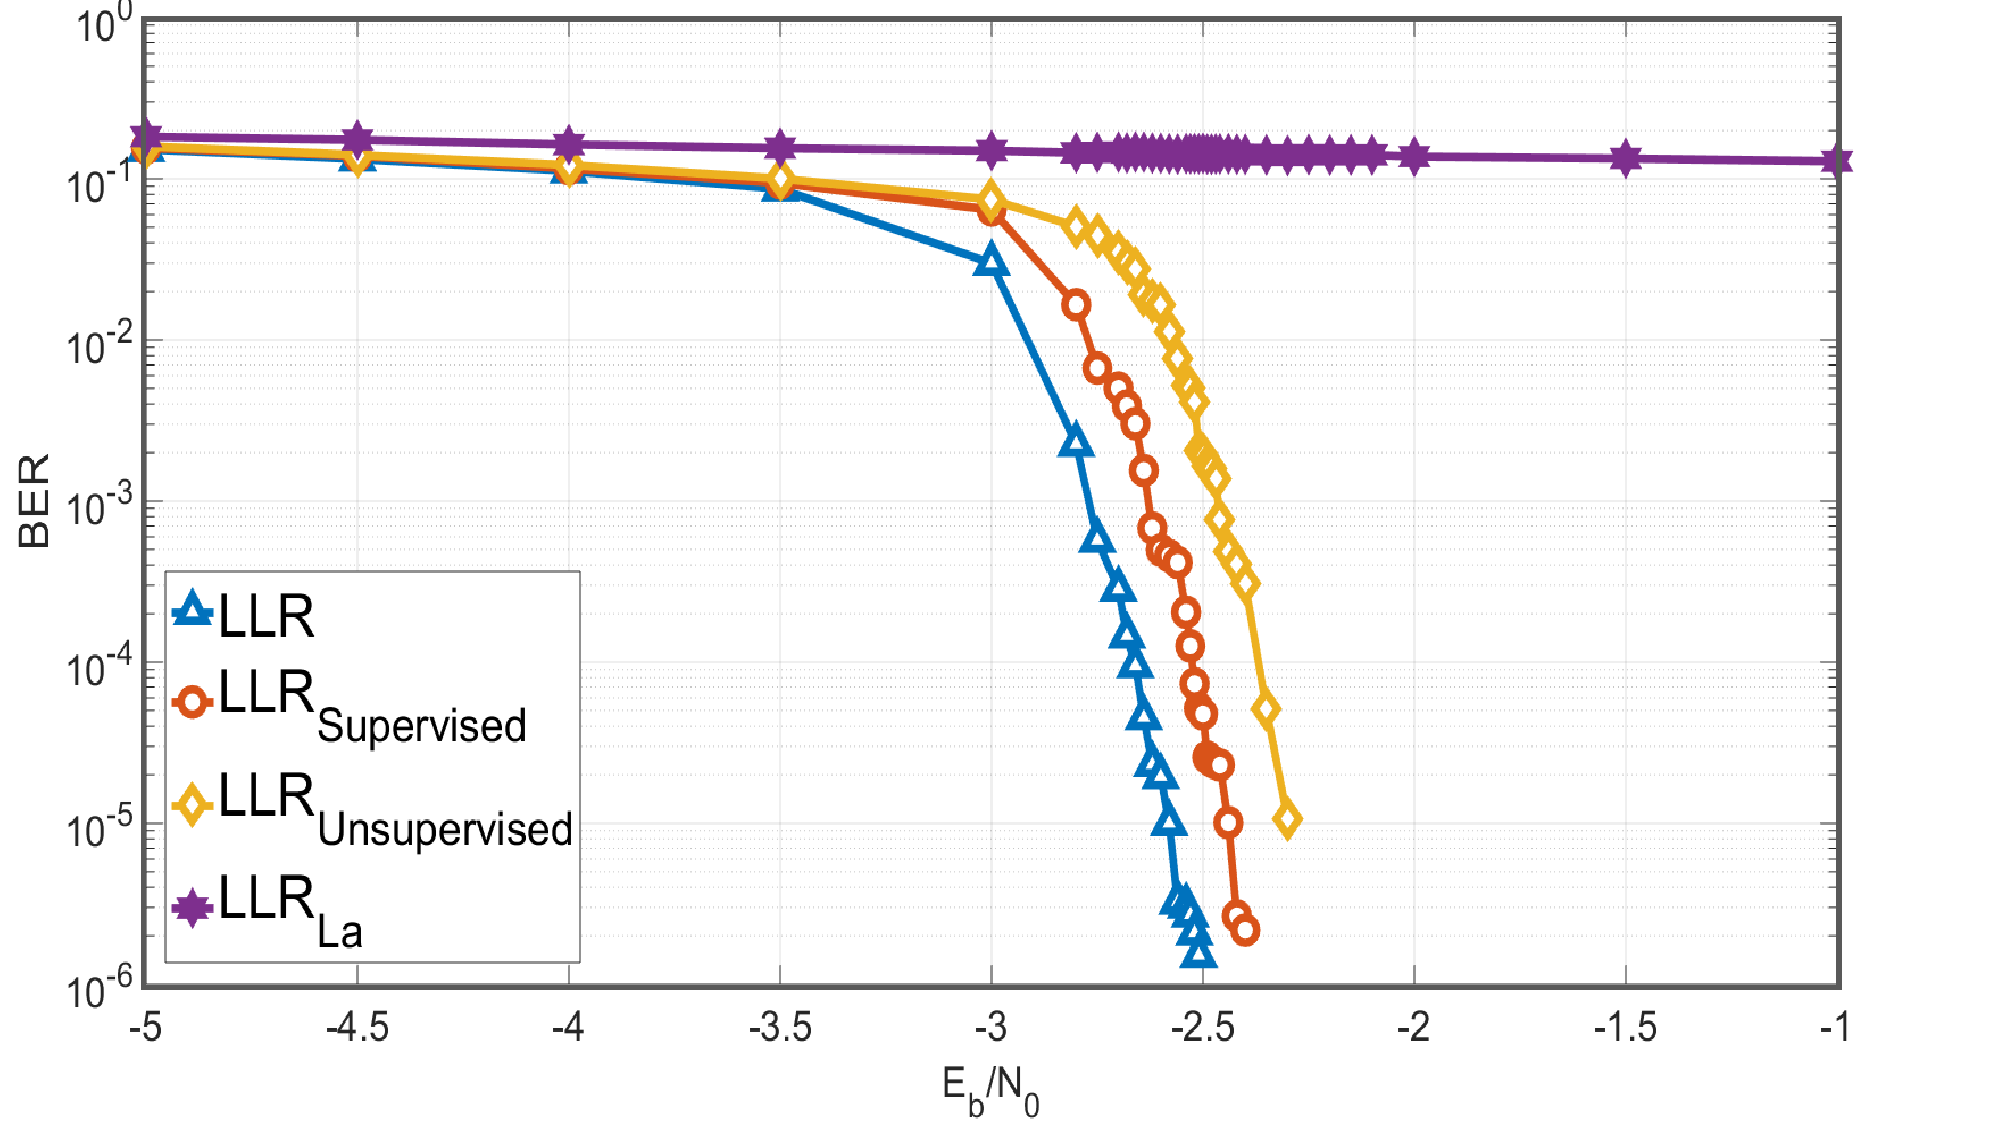
\includegraphics[width=\linewidth]{fig-15}
  \caption{BER comparison as a function of $E_b/N_0$ between
    the supervised, unsupervised, Gaussian designed LLR
    approximations and the LLR obtained by numerical
    integration, in highly impulsive
    $\varepsilon$-Contaminated noise with $\varepsilon=0.1$
    and $K=10$.}
  \label{fig:15}
\end{figure}

\begin{figure}
  \centering 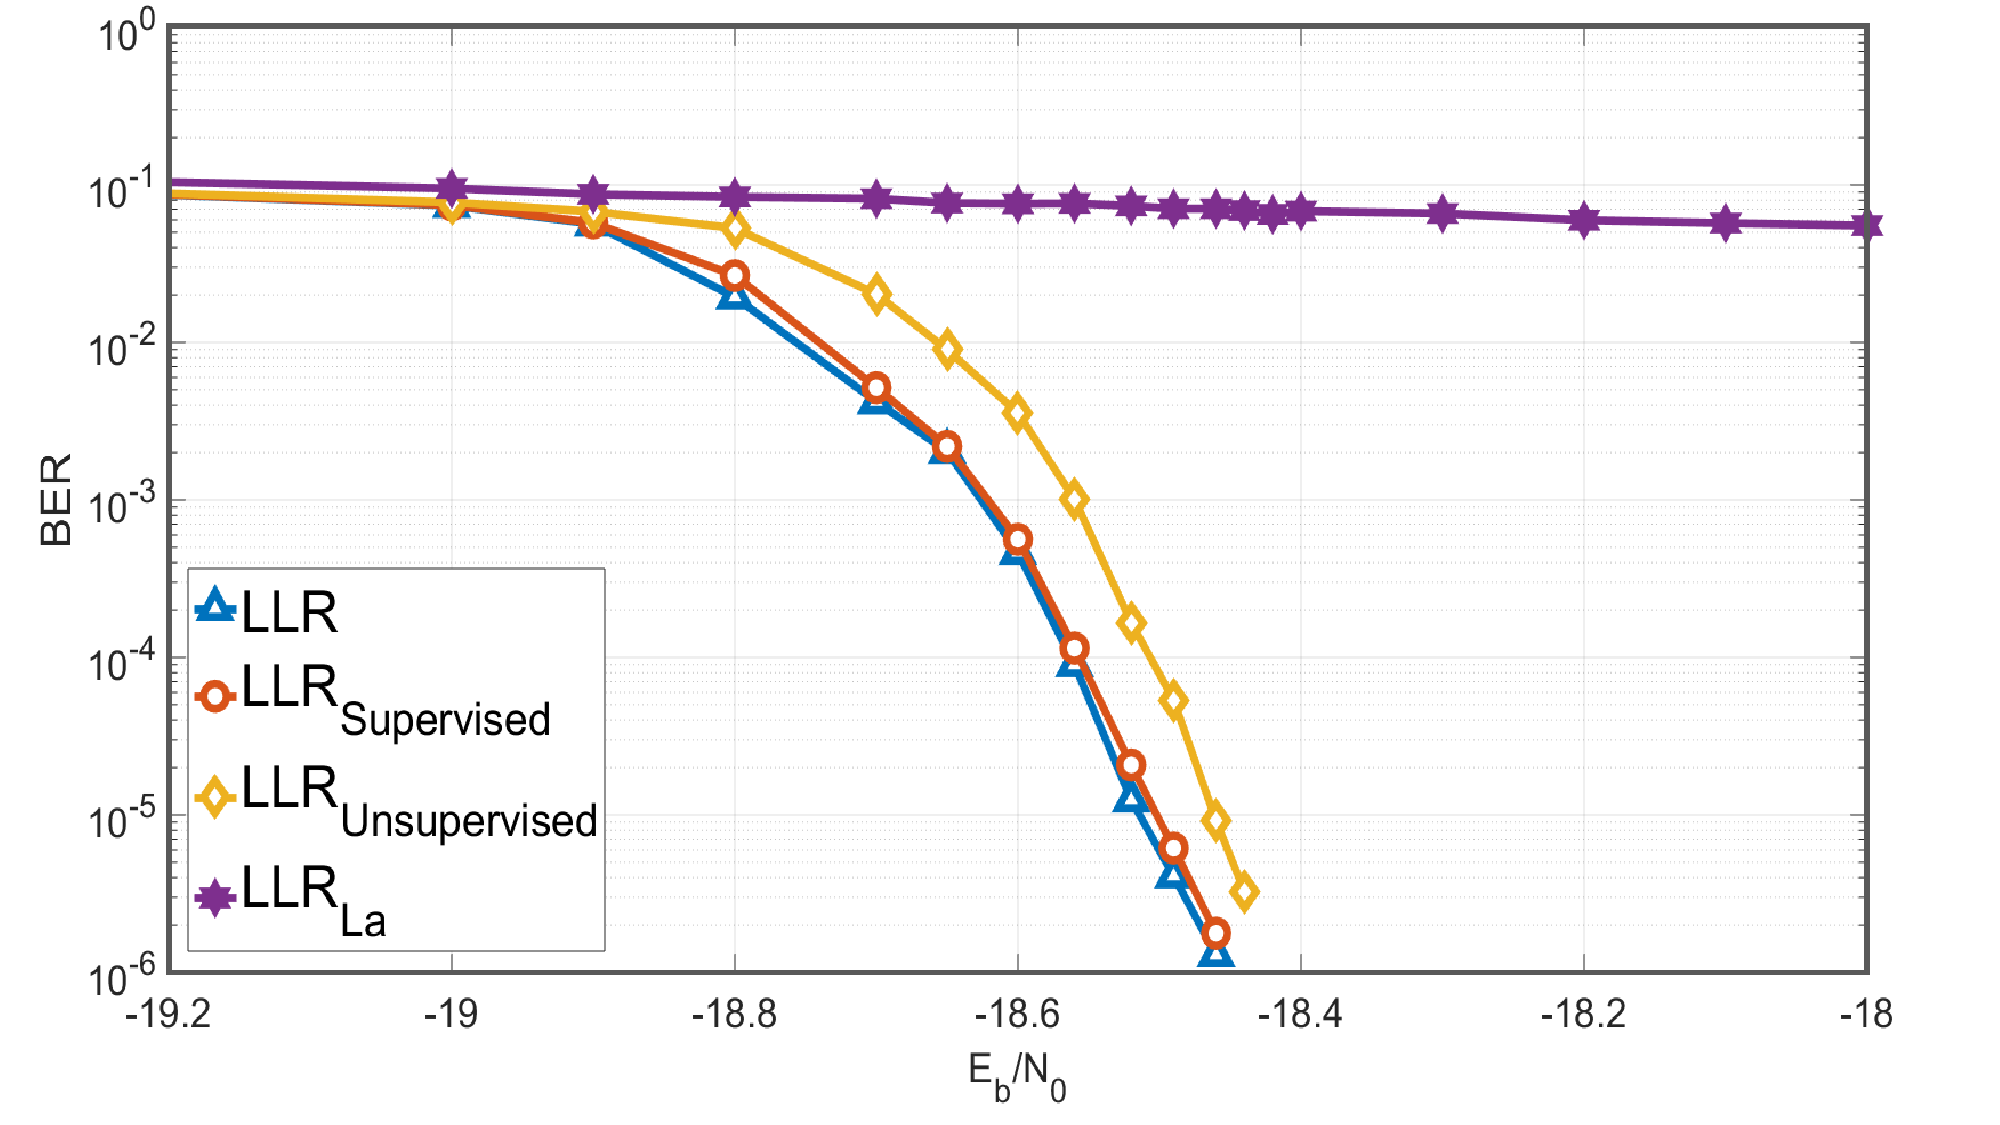
\includegraphics[width=\linewidth]{fig-16}
  \caption{BER comparison as a function of $E_b/N_0$ between
    the supervised, unsupervised, Gaussian designed LLR
    approximations and the LLR obtained by numerical
    integration, in poorly impulsive Middleton Class A noise
    with $ A=0.01$ and $\Gamma=0.01$.}
  \label{fig:16}
\end{figure}

\begin{figure}
  \centering 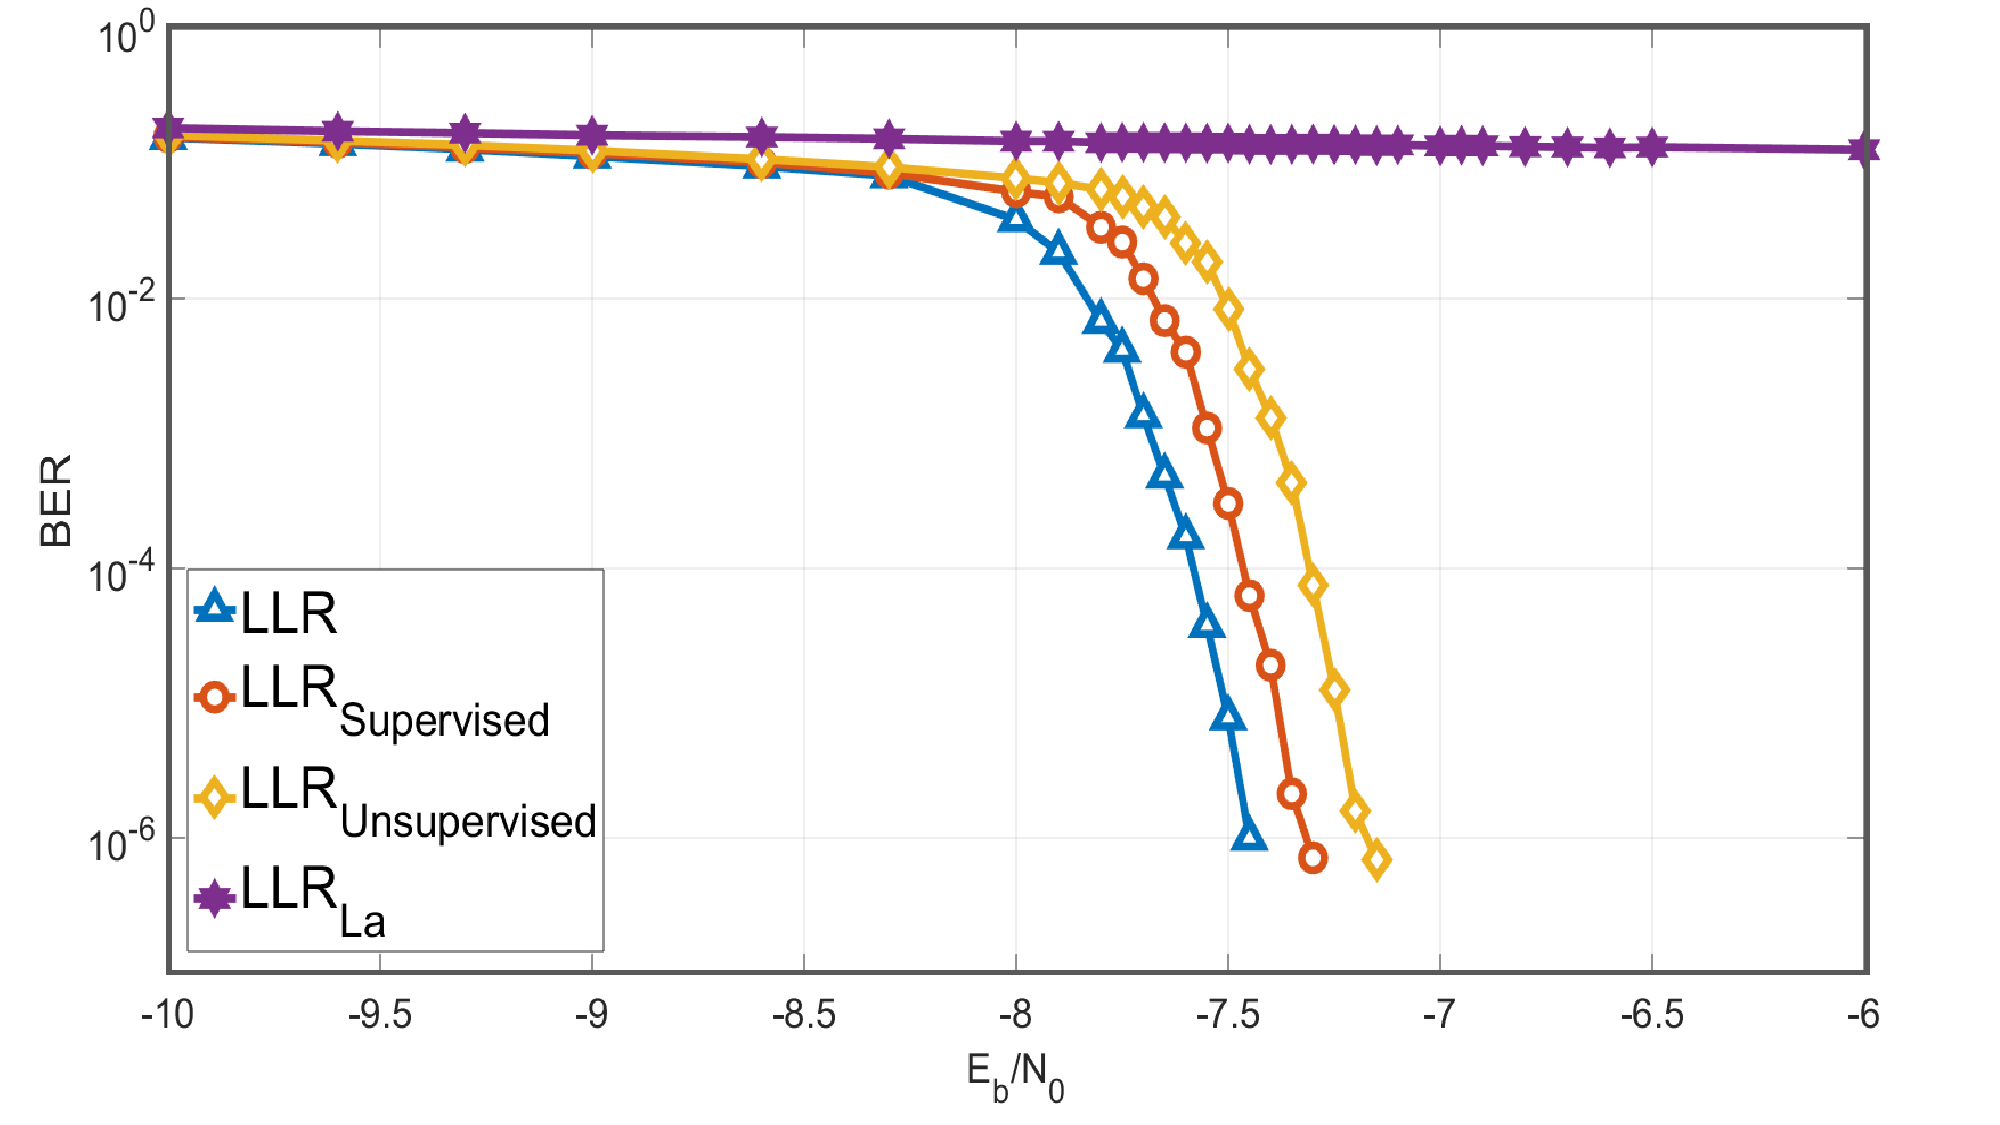
\includegraphics[width=\linewidth]{fig-17}
  \caption{BER comparison as a function of $E_b/N_0$ between
    the supervised, unsupervised, Gaussian designed LLR
    approximations and the LLR obtained by numerical
    integration, in highly impulsive Middleton Class A noise
    with $A=0.1$ and $\Gamma=0.1$.}
  \label{fig:17}
\end{figure}

The high robustness of our demapper can be seen through the
close performance obtained between the blind and supervised
case from one side, and between both approximations to the
true LLR from the other side in spite of the change of the
type of noise.

\textcolor{red}{A: In the following, we will investigate the
  performance of our proposed demapper under Gaussian
  noise. }


\subsubsection{Additive Gaussian noise channel}


\textcolor{red}{A: Since the Gaussian case is an extreme
  case of a $S\alpha S$ noise with $\alpha=2$, we whish to
  check if the performance of our decoding scheme is not
  degraded when the channel suffers a purely Gaussian
  noise.}

The approximated LLR $L_{a,b}$ is thus tested in the
presence of a Gaussian noise and \textcolor{red}{the
  obtained BER is} shown in \figurename~\ref{fig:18}.

\begin{figure}
  \centering
  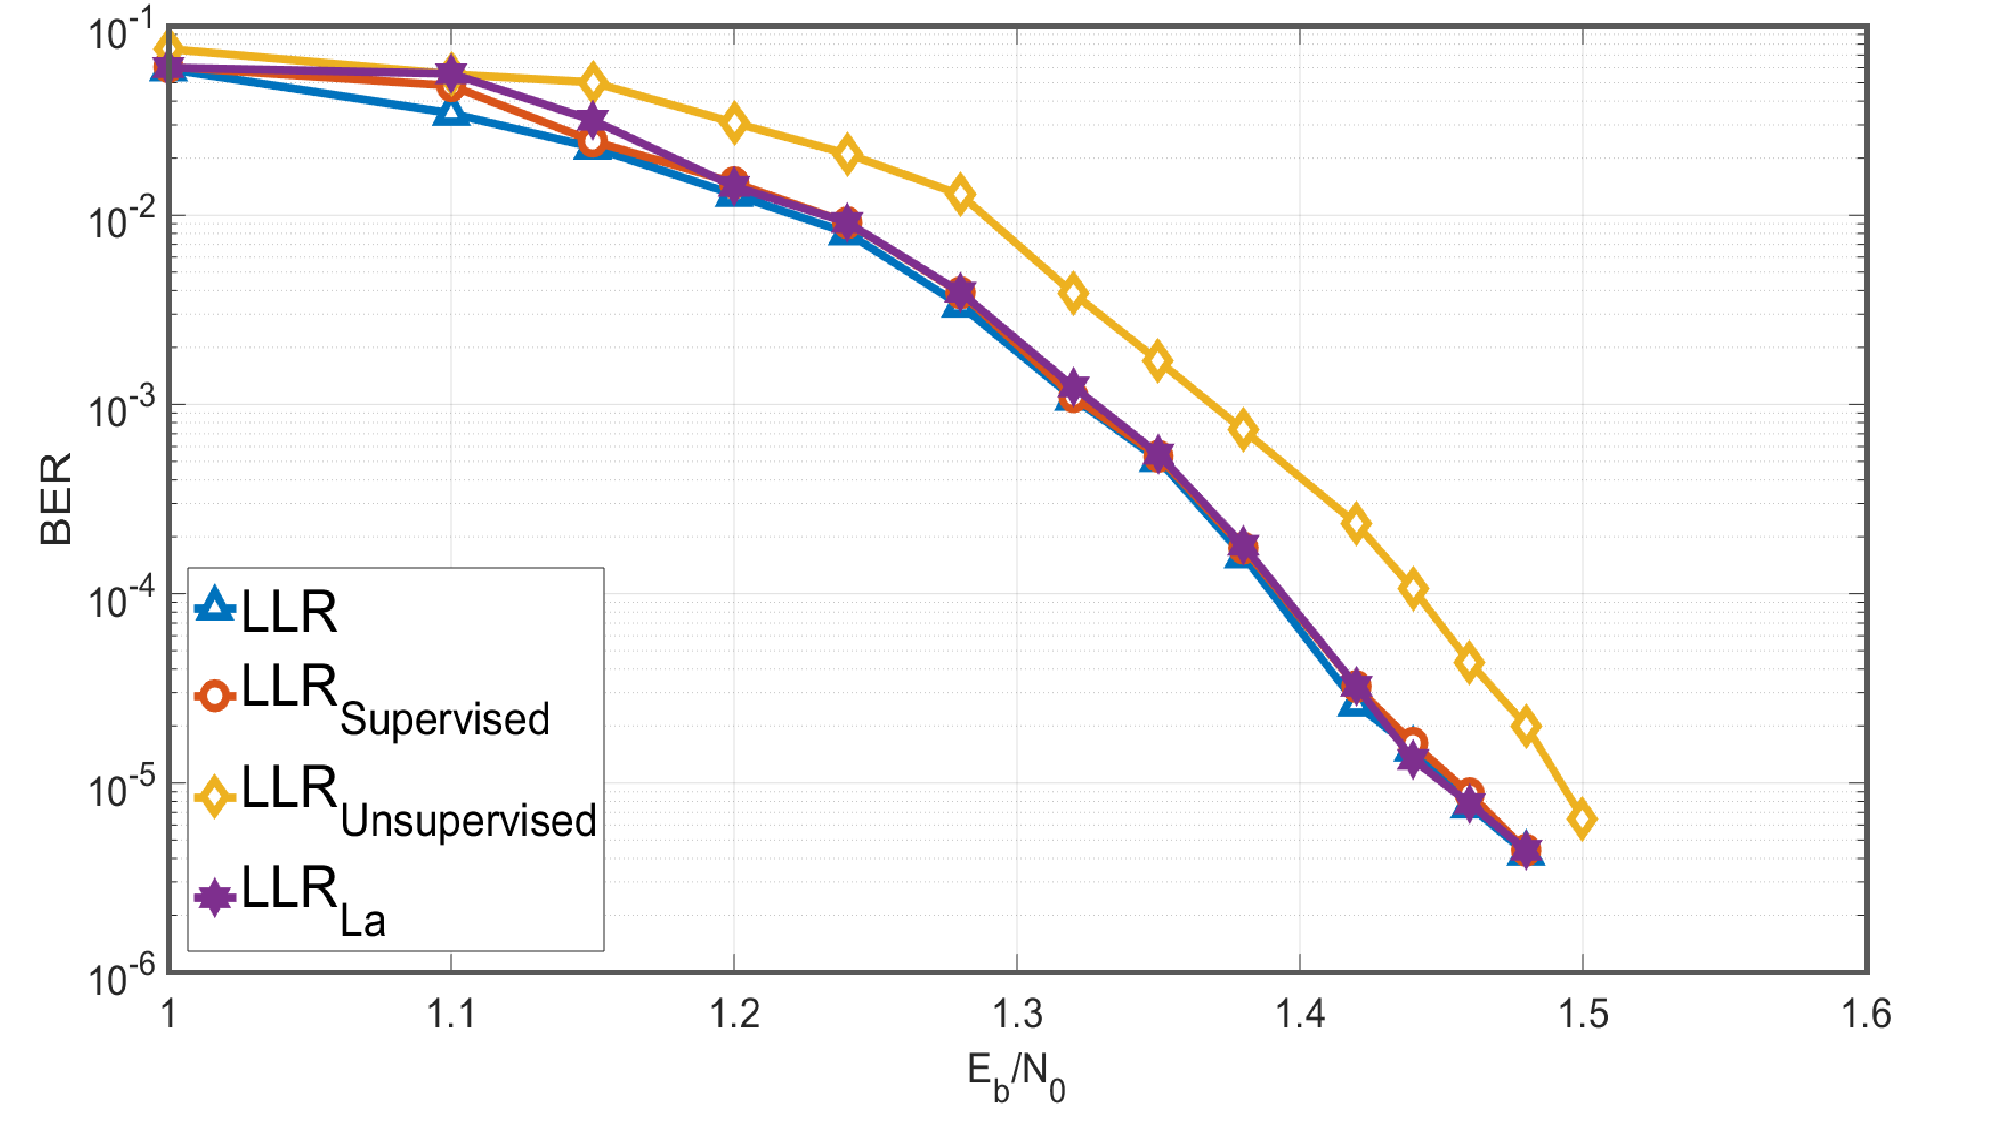
\includegraphics[width=\linewidth]{fig-18}
  \caption{BER comparison as a function of $E_b/N_0$ between
    the supervised, unsupervised LLR approximations and the
    optimal LLR.}
  \label{fig:18}
\end{figure}

\textcolor{red}{Since all curves, i.e.\ the BER obtained
  under both the supervised and blind optimization, as well
  as the optimal demapper $L_a^*$ for Gaussian noise and the
  one obtained with the true LLR, are almost
  \textcolor{blue}{superposed (why the gap under unsup??)},
  our proposed approach with the optimized $L_{a,b}$ does
  not degrade the decoding performance in a purely Gaussian
  case.}


\subsubsection{Analysis}

These numerical simulations illustrate the universality of
the approach. The LLR family has to be wide enough to be
able to represent the linear behavior of exponential-tail
noises like the Gaussian and the non-linear behavior of
sub-exponential distributions of the impulsive noises. The
estimation of the LLR approximation parameter rely on an
information theory criteria which does not depend on any
noise assumption nor function to be estimated. As long as
the approximation family ensures the convexity of the
optimization problem, a solution will exist and will be
efficient in the communication context.

The gap between the blind optimization and the true LLR is
of the order of 0.3 dB in the worst case, showing the
strength of the blind optimized demapper. Moreover, one can
achieve an enormous gap within the range [9.5-15] dB between
$L_{ab}$ and $L_a$, showing the influence of handling
correctly the impulses that arise due to the presence of
interference. Moreover, our demapper function does not
impact the performance if you do not have impulsive noise so
that we do not need a detection step to distinguish between
Gaussian or impulsive noise.





\section{Conclusion}
\label{section:conclu}

We proposed in this paper a Universal receiver design. We
use an LLR approximation function $f_\theta$ in a parametric
family. The parameters $\theta$ are estimated through the
maximization of the mutual information. A blind solution is
proposed in order to benefit form the whole received
sequence but also to increase the useful data rate. Our
results show that the receiver design is efficient in
a large variety of noises and that the blind estimation
allows to reach performance close to the optimal and better
than the supervised approach if a reasonable training
sequence length is considered.




\section*{Acknowledgment}
\label{section:Ack}

This work has been partially supported by COST ACTION CA
15104 - IRACON, and IRCICA USR CNRS 3380



\bibliographystyle{IEEEtran}
\bibliography{ReviewedPapers}

\end{document}